% This file was created (at least in part) by the script ParseMdtoLatex by Louis du Plessis
% (Available from https://github.com/taming-the-beast)

\documentclass[11pt]{article}
%%%%%%%%%%%%%%%%%%%%%%%%%%%%%%%%%%%%%%%%%%%%%%%%%%%%%%%%%%%%%%%
% DO NOT EDIT THIS FILE UNLESS YOU KNOW WHAT YOU ARE DOING!!! %
%%%%%%%%%%%%%%%%%%%%%%%%%%%%%%%%%%%%%%%%%%%%%%%%%%%%%%%%%%%%%%%

\usepackage[]{authblk}
\usepackage{graphicx}
\usepackage{color}
\usepackage{longtable}
\usepackage{hanging}
\usepackage{indentfirst}
\usepackage{setspace}
\usepackage{enumitem}
\usepackage{verbatim}
\usepackage{upgreek}
\usepackage{framed}
\usepackage{textcomp}
\usepackage{url}
\usepackage{soul}
\usepackage{amsmath, amsfonts,amssymb,mathrsfs}
\usepackage{fancyhdr}
\usepackage[compact]{titlesec}
\usepackage[T1]{fontenc}
\usepackage{lmodern}

\usepackage[backend=bibtex,hyperref=true,citestyle=authoryear,bibstyle=authortitle,firstinits=true,terseinits=true,doi=false,url=false,eprint=false,maxbibnames=10,maxcitenames=2]{biblatex}
\DeclareCiteCommand{\cite}
  {\usebibmacro{prenote}}
  {\usebibmacro{citeindex}%
   \printtext[bibhyperref]{\usebibmacro{cite}}}
  {\multicitedelim}
  {\usebibmacro{postnote}}

\DeclareCiteCommand*{\cite}
  {\usebibmacro{prenote}}
  {\usebibmacro{citeindex}%
   \printtext[bibhyperref]{\usebibmacro{citeyear}}}
  {\multicitedelim}
  {\usebibmacro{postnote}}

\DeclareCiteCommand{\parencite}[\mkbibparens]
  {\usebibmacro{prenote}}
  {\usebibmacro{citeindex}%
    \printtext[bibhyperref]{\usebibmacro{cite}}}
  {\multicitedelim}
  {\usebibmacro{postnote}}

\DeclareCiteCommand*{\parencite}[\mkbibparens]
  {\usebibmacro{prenote}}
  {\usebibmacro{citeindex}%
    \printtext[bibhyperref]{\usebibmacro{citeyear}}}
  {\multicitedelim}
  {\usebibmacro{postnote}}

\DeclareCiteCommand{\footcite}[\mkbibfootnote]
  {\usebibmacro{prenote}}
  {\usebibmacro{citeindex}%
  \printtext[bibhyperref]{ \usebibmacro{cite}}}
  {\multicitedelim}
  {\usebibmacro{postnote}}

\DeclareCiteCommand{\footcitetext}[\mkbibfootnotetext]
  {\usebibmacro{prenote}}
  {\usebibmacro{citeindex}%
   \printtext[bibhyperref]{\usebibmacro{cite}}}
  {\multicitedelim}
  {\usebibmacro{postnote}}

\DeclareCiteCommand{\textcite}
  {\boolfalse{cbx:parens}}
  {\usebibmacro{citeindex}%
   \printtext[bibhyperref]{\usebibmacro{textcite}}}
  {\ifbool{cbx:parens}
     {\bibcloseparen\global\boolfalse{cbx:parens}}
     {}%
   \multicitedelim}
  {\usebibmacro{textcite:postnote}}

\newcommand{\citep}{\parencite}
\newcommand{\citet}{\textcite}
\defbibheading{relevref}[\refname]{\section*{Relevant References}}

\renewcommand{\postnotedelim}{\iffieldpages{postnote}{\addcolon}{\addcomma\space}} 
\DeclareFieldFormat{postnote}{#1} 

\DeclareFieldFormat[article, inbook, incollection, inproceedings, patent, thesis, unpublished]{title}{#1}
\DeclareFieldFormat[article, inbook, incollection, inproceedings, patent, thesis, unpublished]{journaltitle}{\mkbibemph{#1}\nopunct}
\DeclareFieldFormat[article, inbook, incollection, inproceedings, patent, thesis, unpublished]{volume}{{#1}\addcolon} %puts volume number in parens
%\DeclareFieldFormat[article, inbook, incollection, inproceedings, patent, thesis, unpublished]{year}{\mkbibparens{#1}\nopunct} %puts year in parens

\DeclareFieldFormat[article, incollection, patent, thesis, unpublished]{pages}{{\nopp#1}}

\DeclareFieldFormat{sentencecase}{\MakeSentenceCase{#1}}

\renewbibmacro*{title}{%
  \ifthenelse{\iffieldundef{title}\AND\iffieldundef{subtitle}}
    {}
    {\ifthenelse{\ifentrytype{article}\OR\ifentrytype{inbook}%
      \OR\ifentrytype{incollection}\OR\ifentrytype{inproceedings}%
      \OR\ifentrytype{inreference}}
      {\printtext[title]{%
        \printfield[sentencecase]{title}%
        \setunit{\subtitlepunct}%
        \printfield[sentencecase]{subtitle}}}%
      {\printtext[title]{%
        \printfield[titlecase]{title}%
        \setunit{\subtitlepunct}%
        \printfield[titlecase]{subtitle}}}%
     \newunit}%
  \printfield{titleaddon}}

\DefineBibliographyStrings{english}{% various adjustments to common bib entry strings
urlseen = {Accessed:},% What goes in front of the date a URL was accessed/retrieved etc.
editor = {(Ed)},%Ed – no dot, in brackets
editors = {(Eds)},% Eds – no dot, in brackets
byeditor = {(Ed.)}}% ‘Edited by’ for edited works

\DeclareNameAlias{default}{last-first}

\renewbibmacro{in:}{}

\renewbibmacro{publisher+location+date}{
  \iflistundef{publisher}
    {}
    {\printlist{publisher}%
       {\addcomma\space}%
      \iflistundef{location}
        {}
        {\printlist{location}}%
    }
}

\DeclareBibliographyDriver{article}{%
\usebibmacro{bibindex}%
\usebibmacro{begentry}%
\usebibmacro{author/translator+others}%
\newunit\newblock
\printfield{year}%
\setunit{\labelnamepunct}\newblock
\usebibmacro{title}%
\newunit
\printlist{language}%
\newunit\newblock
\usebibmacro{byauthor}%
\newunit\newblock
\usebibmacro{bytranslator+others}%
\newunit\newblock
\printfield{version}%
\newunit\newblock
%\usebibmacro{in:}% %mit in:
\usebibmacro{journal}%
\newunit\newblock
\printfield{volume}%
\newunit\newblock
\usebibmacro{byeditor+others}%
\newunit\newblock
\usebibmacro{note+pages}%
\newunit\newblock
\iftoggle{bbx:isbn}
{}%
\newunit\newblock
\usebibmacro{doi+eprint+url}%
\newunit\newblock
\usebibmacro{addendum+pubstate}%
\newunit\newblock
\usebibmacro{pageref}%
\usebibmacro{finentry}}

\DeclareBibliographyDriver{inproceedings}{%
\usebibmacro{bibindex}%
\usebibmacro{begentry}%
\usebibmacro{author/translator+others}%
\newunit\newblock
\printfield{year}%
\setunit{\labelnamepunct}\newblock
\usebibmacro{title}%
\newunit
\printlist{language}%
\newunit\newblock
\usebibmacro{byauthor}%
\newunit\newblock
\usebibmacro{bytranslator+others}%
\newunit\newblock
\printfield{version}%
\newunit\newblock
%\usebibmacro{in:}% %mit in:
\usebibmacro{booktitle}%
\newunit\newblock
\printfield{volume}%
\newunit\newblock
\usebibmacro{byeditor+others}%
\newunit\newblock
\usebibmacro{publisher+location+date}%
\newunit\newblock
\usebibmacro{note+pages}%
\newunit\newblock
\usebibmacro{pageref}%
\usebibmacro{finentry}}

\DeclareBibliographyDriver{book}{%
\usebibmacro{bibindex}%
\usebibmacro{begentry}%
\usebibmacro{author/translator+others}%
\newunit\newblock
\printfield{year}%
\setunit{\labelnamepunct}\newblock
\usebibmacro{title}%
\newunit
\printlist{language}%
\newunit\newblock
\usebibmacro{byauthor}%
\newunit\newblock
\usebibmacro{bytranslator+others}%
\newunit\newblock
%\usebibmacro{in:}% %mit in:
\usebibmacro{booktitle}%
\newunit\newblock
\printfield{volume}%
\newunit\newblock
\usebibmacro{publisher+location+date}%
\newunit\newblock
\usebibmacro{note+pages}%
\newunit\newblock
\usebibmacro{pageref}%
\usebibmacro{finentry}}




\setlist{nolistsep}

\setlength{\evensidemargin}{0in}
\setlength{\headheight}{0in}
\setlength{\headsep}{0in}
\setlength{\oddsidemargin}{-0.25in}
\setlength{\paperheight}{11in}
\setlength{\paperwidth}{8.5in}
\setlength{\tabcolsep}{0in}
\setlength{\textheight}{9in}
\setlength{\textwidth}{7in}
\setlength{\topmargin}{0in}
\setlength{\topskip}{0in}
\setlength{\voffset}{0in}
\parskip = 0.15in
\pagestyle{plain}
\setlength{\parindent}{0cm}

\definecolor{citescol}{RGB}{194,101,1}
\definecolor{urlscol}{RGB}{0,150,206}
\definecolor{linkscol}{RGB}{149,0,207}
\definecolor{mycol}{RGB}{25,23,191}
\definecolor{outputcol}{RGB}{34,139,34}
\definecolor{tcol}{RGB}{165,0,14}


\DeclareMathAlphabet{\msfsl}{T1}{cmr}{m}{it}
\DeclareMathAlphabet{\msyf}{OMX}{pcr}{m}{it}
\newcommand{\alf}{\upalpha}
\newcommand{\hilight}[1]{\colorbox{yellow}{#1}}

\newcommand{\levelone}[1]{
\bigskip
\noindent{\LARGE{\textsc{#1}}}
\vspace {0.05in}
}

\newcommand{\leveltwo}[1]{
\bigskip
\noindent{\Large{\textit{#1}}}
\vspace {-1mm}
}

\newcommand{\descriptionhead}[1]{
\noindent{\textcolor{mycol}{\textbf{\textit{#1}}}}\\ \vspace{-7mm}
}

\newcommand{\dhead}[1]{
\noindent{\textbf{\textit{#1 --}}}
}



\newcommand{\exs}[1]{
\vspace{-4mm}
\begin{itemize}
\item #1 \\ \vspace{-8mm}
\end{itemize}
}

\newcommand{\nbo}[1]{{\color{red}{#1}}}


\newcommand{\stepbullet}{\noindent \textbullet \ }
\newcommand{\mi}[1]{\textbf{\textit{#1}}}


\newcommand{\levelthree}[1]{\textit{#1 --}}


%\bibliographystyle{apalike}
%\bibpunct[; ]{(}{)}{;}{a}{,}{;}


\usepackage[breaklinks]{hyperref}
\usepackage[all]{hypcap}
\hypersetup{colorlinks=true,linkcolor=linkscol,citecolor=citescol,urlcolor=urlscol}


\newcommand{\R}{\texttt{R} }
\newcommand{\TESS}{\texttt{TESS}}
\newcommand{\PBD}{\texttt{PBD}}
\newcommand{\DDD}{\texttt{DDD}}
\newcommand{\Laser}{\texttt{laser}}
\newcommand{\TreePar}{\texttt{TreePar}}
\newcommand{\diversitree}{\texttt{diversitree}}
\newcommand{\RevBayes}{\texttt{RevBayes}}
\newcommand{\Rev}{\texttt{Rev}}
\newcommand{\MrBayes}{\texttt{MrBayes}}
\newcommand{\BEAST}{\texttt{BEAST}}
\newcommand{\PhyloBayes}{\texttt{PhyloBayes}}
\newcommand{\PAML}{\texttt{PAML}}

\let\otheriint\iint
\let\iint\relax
\usepackage{ wasysym }

\usepackage{framed}
\usepackage[]{listings}
%\usepackage{fontspec}
\usepackage{placeins}
\usepackage{epstopdf}



\lstset{backgroundcolor=\color[rgb]{0.972,0.972,0.972},
		tabsize=4,
		rulecolor=,
        basicstyle=\scriptsize,
        upquote=true,
        aboveskip={1.5\baselineskip},
        columns=fixed,
        showstringspaces=false,
        extendedchars=true,
        breaklines=true,
        prebreak = \raisebox{0ex}[0ex][0ex]{\ensuremath{\hookleftarrow}},
        frame=single,
        showtabs=false,
        showspaces=false,
        showstringspaces=false,
        identifierstyle=\ttfamily,
        keywordstyle=\color[rgb]{0,0,1},
        commentstyle=\color[rgb]{0.133,0.545,0.133},
        stringstyle=\color[rgb]{0.627,0.126,0.941}
}

\definecolor{shadecolor}{RGB}{194,225,255}

\setlength{\tabcolsep}{5pt}
\setlength{\topmargin}{-0.4in}
\setlength{\headheight}{14.5pt}
\pagestyle{fancy}

\newcommand{\taha}[1]{{\textcolor{red}{[TAH comment: #1]}}} % TAH comment

\titlespacing{\section}{0pt}{*0}{*0}
\titlespacing{\subsection}{0pt}{*0}{*0}
\titlespacing{\subsubsection}{0pt}{*0}{*0}

\titleformat{\section}
  {\normalfont\Large\bfseries\color{mycol}}
  {\thesection}{1em}{}

\titleformat{\subsection}
  {\normalfont\large\bfseries\color{mycol}}
  {\thesubsection}{1em}{}

\titleformat{\subsubsection}
  {\normalfont\bfseries\color{mycol}}
  {\thesubsubsection}{1em}{}

% command for MrBayes command-line step
\newcommand{\cl}[1]{{\texttt{\textbf{#1}}}}

\newcommand{\colx}[1]{{\textcolor{tcol}{#1}}}

\newcommand{\mbcl}[1]{\exs{\cl{MrBayes > {#1}}}}

\newcommand{\rbprmt}{RevBayes > } 
\newcommand{\rbcl}[1]{\exs{\cl{\rbprmt{#1}}}}
\newcommand{\rbout}[1]{\exs{\cl{\textcolor{outputcol}{#1}}}}
\newcommand{\rbdn}{{\Large \symbol{126}}} % This makes a copy/pasteable tilde
\newcommand{\rbclml}[1]{\exs{\cl{\ \ \ \ \ \ \ \ \ \ \ {#1}}}}

% text box settings
% requires compiling w/ XeLaTeX
%\newfontfamily\listingsfont[Scale=1.0]{Courier New}
%\lstset{basicstyle=\listingsfont, columns=texcl}
%\defaultfontfeatures{Mapping=tex-text}


\makeatletter
\lst@CCPutMacro\lst@ProcessOther {"2D}{\lst@ttfamily{-{}}{-{}}}
\@empty\z@\@empty
\makeatother


\usepackage{tikz}

\setlength{\topmargin}{-0.4in}
\setlength{\headheight}{14.5pt}
\pagestyle{fancy}

\usepackage[breaklinks]{hyperref}
\usepackage[all]{hypcap}
\hypersetup{colorlinks=true,linkcolor=linkscol,citecolor=citescol,urlcolor=urlscol}

\definecolor{lg}{gray}{0.75}
\def\gcirc{{%
    \setbox0\hbox{$\fullmoon$}%
    \rlap{\hbox to \wd0{\hss{$\textcolor{lg}{\newmoon}$}\hss}}\box0
}}



% Add your bibtex library here
\addbibresource{master-refs}


%%%%%%%%%%%%%%%%%%%%
% Do NOT edit this %
%%%%%%%%%%%%%%%%%%%%
\begin{document}
\renewcommand{\headrulewidth}{0.5pt}
\headsep = 20pt
\lhead{ }
\rhead{\textsc {BEAST v2 Tutorial}}
\thispagestyle{plain}


%%%%%%%%%%%%%%%%%%
% Tutorial title %
%%%%%%%%%%%%%%%%%%
\begin{center}

	% Enter the name of your tutorial here
	\textbf{\LARGE Tutorial using BEAST v2.4.7}\\\vspace{2mm}

	% Enter a short description of your tutorial here
	\textbf{\textcolor{mycol}{\Large SCOTTI Tutorial}}\\

	\vspace{4mm}

	% Enter the names of all the authors here
	{\Large {\em Louis du Plessis and Nicola de Maio}}
\end{center}

Transmission tree reconstruction with the structured coalescent

%%%%%%%%%%%%%%%%%
% Tutorial body %
%%%%%%%%%%%%%%%%%

\section{Background}\label{background}

When applying phylodynamic models to pathogen genetic sequences
collected during an outbreak, we usually make the assumption that the
inferred genealogy approximates the true transmission tree. In most
cases the structure of the true transmission tree will be similar to the
inferred genealogy and inferences about epidemiological parameters
(e.g.~the $ R_e $) are valid. However, due to complicating
factors, such as within-host diversity and evolution, non-sampled
patients and transmission bottlenecks, it is difficult to reconstruct
transmission chains or draw conclusions about the transmission dynamics
between infected patients. In particular, there may be discrepancies
between the epidemiological and phylogenetic relatedness of hosts and
infection times are often biased.

SCOTTI (Structured COalescent Transmission Tree Inference)
\citep{deMaio2016} is a BEAST2 package that was developed to provide
more accurate reconstructions of transmission trees. The underlying
model is a structured coalescent model, where each host is modeled as a
population and migrations between populations represent new infections.
New sequencing technologies and protocols are making it easier to sample
the within-host diversity of an outbreak and SCOTTI can take advantage
of multiple sequences from each host to better resolve transmission
events. Furthermore, SCOTTI can model non-sampled hosts by dynamically
increasing or decreasing the number of populations (hosts). (In other
structured models available in BEAST2 the number of populations remain
constant and each population needs to be represented by at least one
sampled sequence). In addition to genetic sequences, SCOTTI also uses
epidemiological data about host exposure times, only allowing hosts to
transmit the disease during periods when they are infectious. Thus,
SCOTTI is able to model within-host diversity as well as non-sampled
hosts and multiply infected hosts. However, it is currently not able to
model transmission bottlenecks.

To make the inference tractable SCOTTI uses the same techniques as BASTA
\citep{deMaio2015}, which is a computationally efficient approximation
to the structured coalescent. In addition, a number of simplifying
assumptions are made. It is assumed that all hosts have the same
infection rate and that it stays constant over the course of infection.
It is also assumed that infection is equally likely between every pair
of hosts. Finally, it is assumed that all hosts have the same effective
population size, $ N_e $. Thus, all hosts have the same
within-host genetic diversity and thus all hosts have equal and constant
within-host dynamics. \clearpage

\section{Programs used in this
Exercise}\label{programs-used-in-this-exercise}

\subsubsection{BEAST2 - Bayesian Evolutionary Analysis Sampling Trees
2}\label{beast2---bayesian-evolutionary-analysis-sampling-trees-2}

BEAST2 (\url{http://www.beast2.org}) is a free software package for
Bayesian evolutionary analysis of molecular sequences using MCMC and
strictly oriented toward inference using rooted, time-measured
phylogenetic trees. This tutorial is written for BEAST v2.4.7 \citep{BEAST2book2014}.

\subsubsection{BEAUti2 - Bayesian Evolutionary Analysis
Utility}\label{beauti2---bayesian-evolutionary-analysis-utility}

BEAUti2 is a graphical user interface tool for generating BEAST2 XML
configuration files.

Both BEAST2 and BEAUti2 are Java programs, which means that the exact
same code runs on all platforms. For us it simply means that the
interface will be the same on all platforms. The screenshots used in
this tutorial are taken on a Mac OS X computer; however, both programs
will have the same layout and functionality on both Windows and Linux.
BEAUti2 is provided as a part of the BEAST2 package so you do not need
to install it separately.

\subsubsection{TreeAnnotator}\label{treeannotator}

TreeAnnotator is used to summarise the posterior sample of trees to
produce a maximum clade credibility tree. It can also be used to
summarise and visualise the posterior estimates of other tree parameters
(e.g.~node height).

TreeAnnotator is provided as a part of the BEAST2 package so you do not
need to install it separately.

\subsubsection{Tracer}\label{tracer}

Tracer (\url{http://tree.bio.ed.ac.uk/software/tracer}) is used to
summarise the posterior estimates of the various parameters sampled by
the Markov Chain. This program can be used for visual inspection and to
assess convergence. It helps to quickly view median estimates and 95\%
highest posterior density intervals of the parameters, and calculates
the effective sample sizes (ESS) of parameters. It can also be used to
investigate potential parameter correlations. We will be using Tracer
v1.6.0.

\subsubsection{FigTree}\label{figtree}

FigTree (\url{http://tree.bio.ed.ac.uk/software/figtree}) is a program
for viewing trees and producing publication-quality figures. It can
interpret the node-annotations created on the summary trees by
TreeAnnotator, allowing the user to display node-based statistics
(e.g.~posterior probabilities). We will be using FigTree v1.4.3.

\subsubsection{Python}\label{python}

Python (\url{https://www.python.org}) is an interpreted programming
language that is often used to write scripts for processing text files.
We will use two Python scripts during the tutorial. Both scripts should
work with Python 2.7.x and Python 3.x. There is also a third, optional,
script that makes use of the \lstinline!graph-tool! package to produce a
better looking figure.

Python should already be installed on most Mac OS X or Linux systems.
Both graphviz and graph-tool are available on Homebrew, and graphviz can
also be installed using \lstinline!apt-get! on Linux systems.

\clearpage

\section{Practical: SCOTTI tutorial}\label{practical-scotti-tutorial}

In this tutorial we analyse an outbreak of Foot and Mouth Disease Virus
(FMDV) that occurred in the South of England in 2007. FMDV is a highly
infectious disease that affects cloven-hoofed animals (such as cattle,
sheep, pigs, deer etc.) and can be easily spread between farms through
contact with contaminated vehicles or animal feed. The usual response to
FMDV is to cull all exposed livestock and quarantine surrounding farms,
thus the effects of the disease can be devastating to the farming sector
(the 2001 outbreak in the United Kingdom resulted in the culling of more
than 10 million cows and sheep and cost £8 billion). It is therefore
extremely important to trace the source and spread of the disease
between farms. Because of the high genetic variability of FMDV an
appreciable amount of genetic variation will accumulate over the course
of an outbreak. Thus, epidemiological and evolutionary dynamics occur on
the same timescale and we are dealing with a measurably evolving
population, which we can analyse in BEAST.

When analysing an FMDV outbreak we can treat each infected farm as an
infected host, with the transmission tree describing infections between
farms. In fact, when discussing livestock diseases it is common to refer
to infected farms as cases, instead of individual infected animals.
(This analogy holds because the genetic diversity of the virus within a
farm is much lower than between farms, thus each farm behaves more like
a single host).

\subsection{The Data}\label{the-data}

We analyse an outbreak of Foot and Mouth Disease Virus (FMDV) that
occurred in the South of England. The outbreak contained two distinct
clusters, in August and September of 2007, respectively. The dataset
contains 11 viral sequences from 10 farms. Four sequences were sampled
during the first cluster and a further 7 during the second cluster. In
addition, we also have the earliest and latest possible dates during
which each farm was infected with the disease, informed by the culling
time and first appearance of symptoms (Figure \ref{fig:outbreak}). The
data were first analysed in \citep{Cottam2008PlosPath} and later
reanalysed using SCOTTI in \citep{deMaio2016}.

\begin{figure}
    \centering
    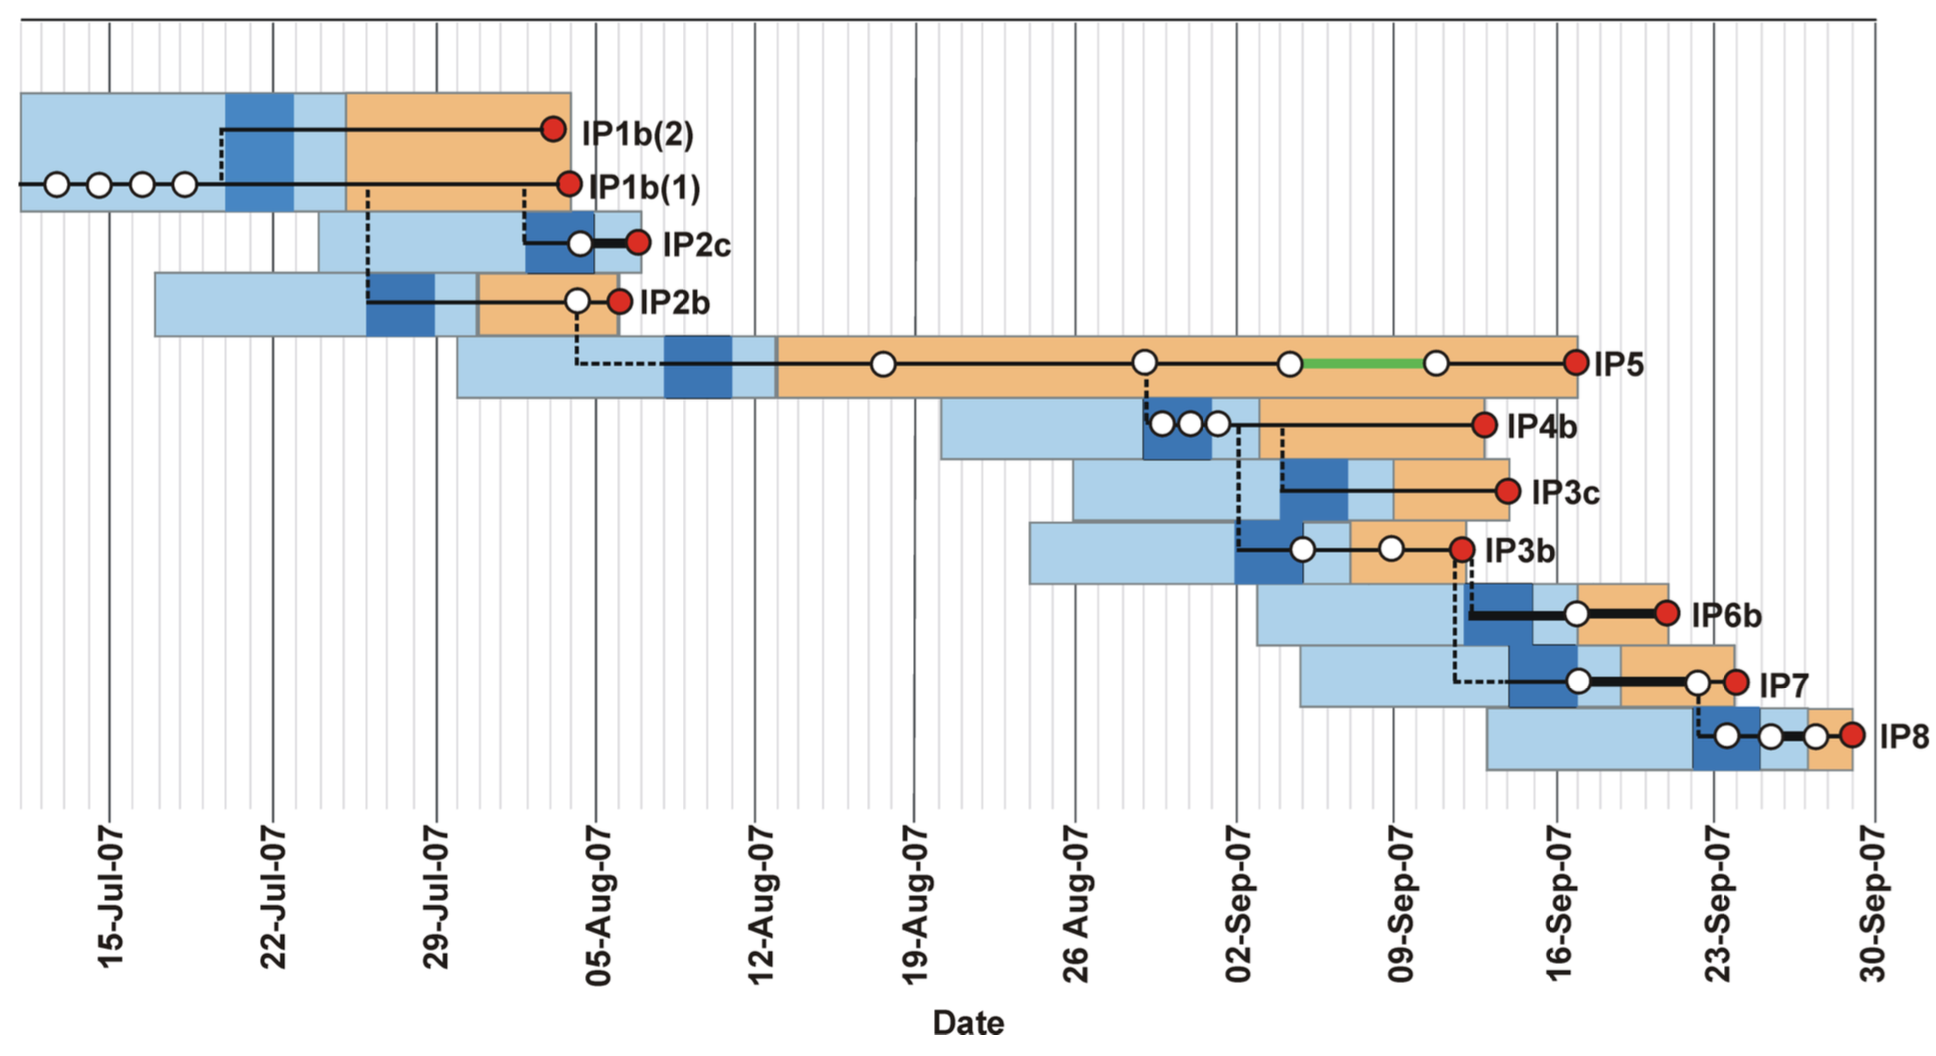
\includegraphics[width=0.800000\textwidth]{figures/Outbreak.png}
    \caption{Exposure times of infected farms and sampling dates of the viral sequences (Figure taken from \citep{Cottam2008PlosPath}). The orange shading estimates the time when animals showing symptoms of FMDV were present on a farm. Light blue shading indicates estimates for the incubation time of each farm. The dark blue shading is the infection date estimates in \citep{Cottam2008PlosPath}. The haplotype network of the sequenced strains is superimposed on the exposure times. The red dots indicate the dates of the sampled sequences.}
    \label{fig:outbreak}
\end{figure}

\subsection{Creating the input files using the included Python
script}\label{creating-the-input-files-using-the-included-python-script}

Unlike most BEAST2 packages, SCOTTI does not have a BEAUti interface.
Although a BEAUti interface makes it much easier, it is not the only way
to create the input XML file for a BEAST2 analysis. Many advanced users
prefer to create the XML file in a text editor as this provides them
with greater flexibility and oversight. Even if you use BEAUti to create
your configuration files it is always a good idea to open the XML file
in a text editor and check that everything is where it should be. At
first glance a BEAST2 XML file may seem bewildering, but the file has a
rigid structure and after a while you will be able to interpret the
different elements of the configuration file. Being able to read and
understand a configuration file gives you a much better understanding of
how the different parts of an analysis fit together. In addition, it
gives you access to models (such as SCOTTI) that do not have BEAUti
interfaces. Once you are familiar with the structure of BEAST2 XML files
and you know the different inputs of the models you want to use you will
find that it is often faster to directly edit an XML file than to create
it in BEAUti.

In this tutorial we we will start at the shallow end of the pool and use
a Python script, \lstinline!SCOTTI_generate_xml.py!, to create the XML
configuration file. It is included with the SCOTTI package and is also
stored in the \lstinline!scripts/! directory of this tutorial.

\subsubsection{Installing the SCOTTI
package}\label{installing-the-scotti-package}

Before we can use SCOTTI we have to install the package somewhere where
BEAST2 can find it. Although we won't use BEAUti to create the input
configuration file, we still have to use BEAUti to install the package.
We will be using SCOTTI version 1.1.1 or above
for this tutorial.

\begin{framed}
Open \textbf{BEAUti} and open the \textbf{BEAST2 Package Manager} by
navigating to \textbf{File \textgreater{} Manage Packages}.

Install \textbf{SCOTTI} by selecting it and clicking the
\textbf{Install/Upgrade} button (Figure \ref{fig:packagemanager})
\end{framed}

\begin{figure}
    \centering
    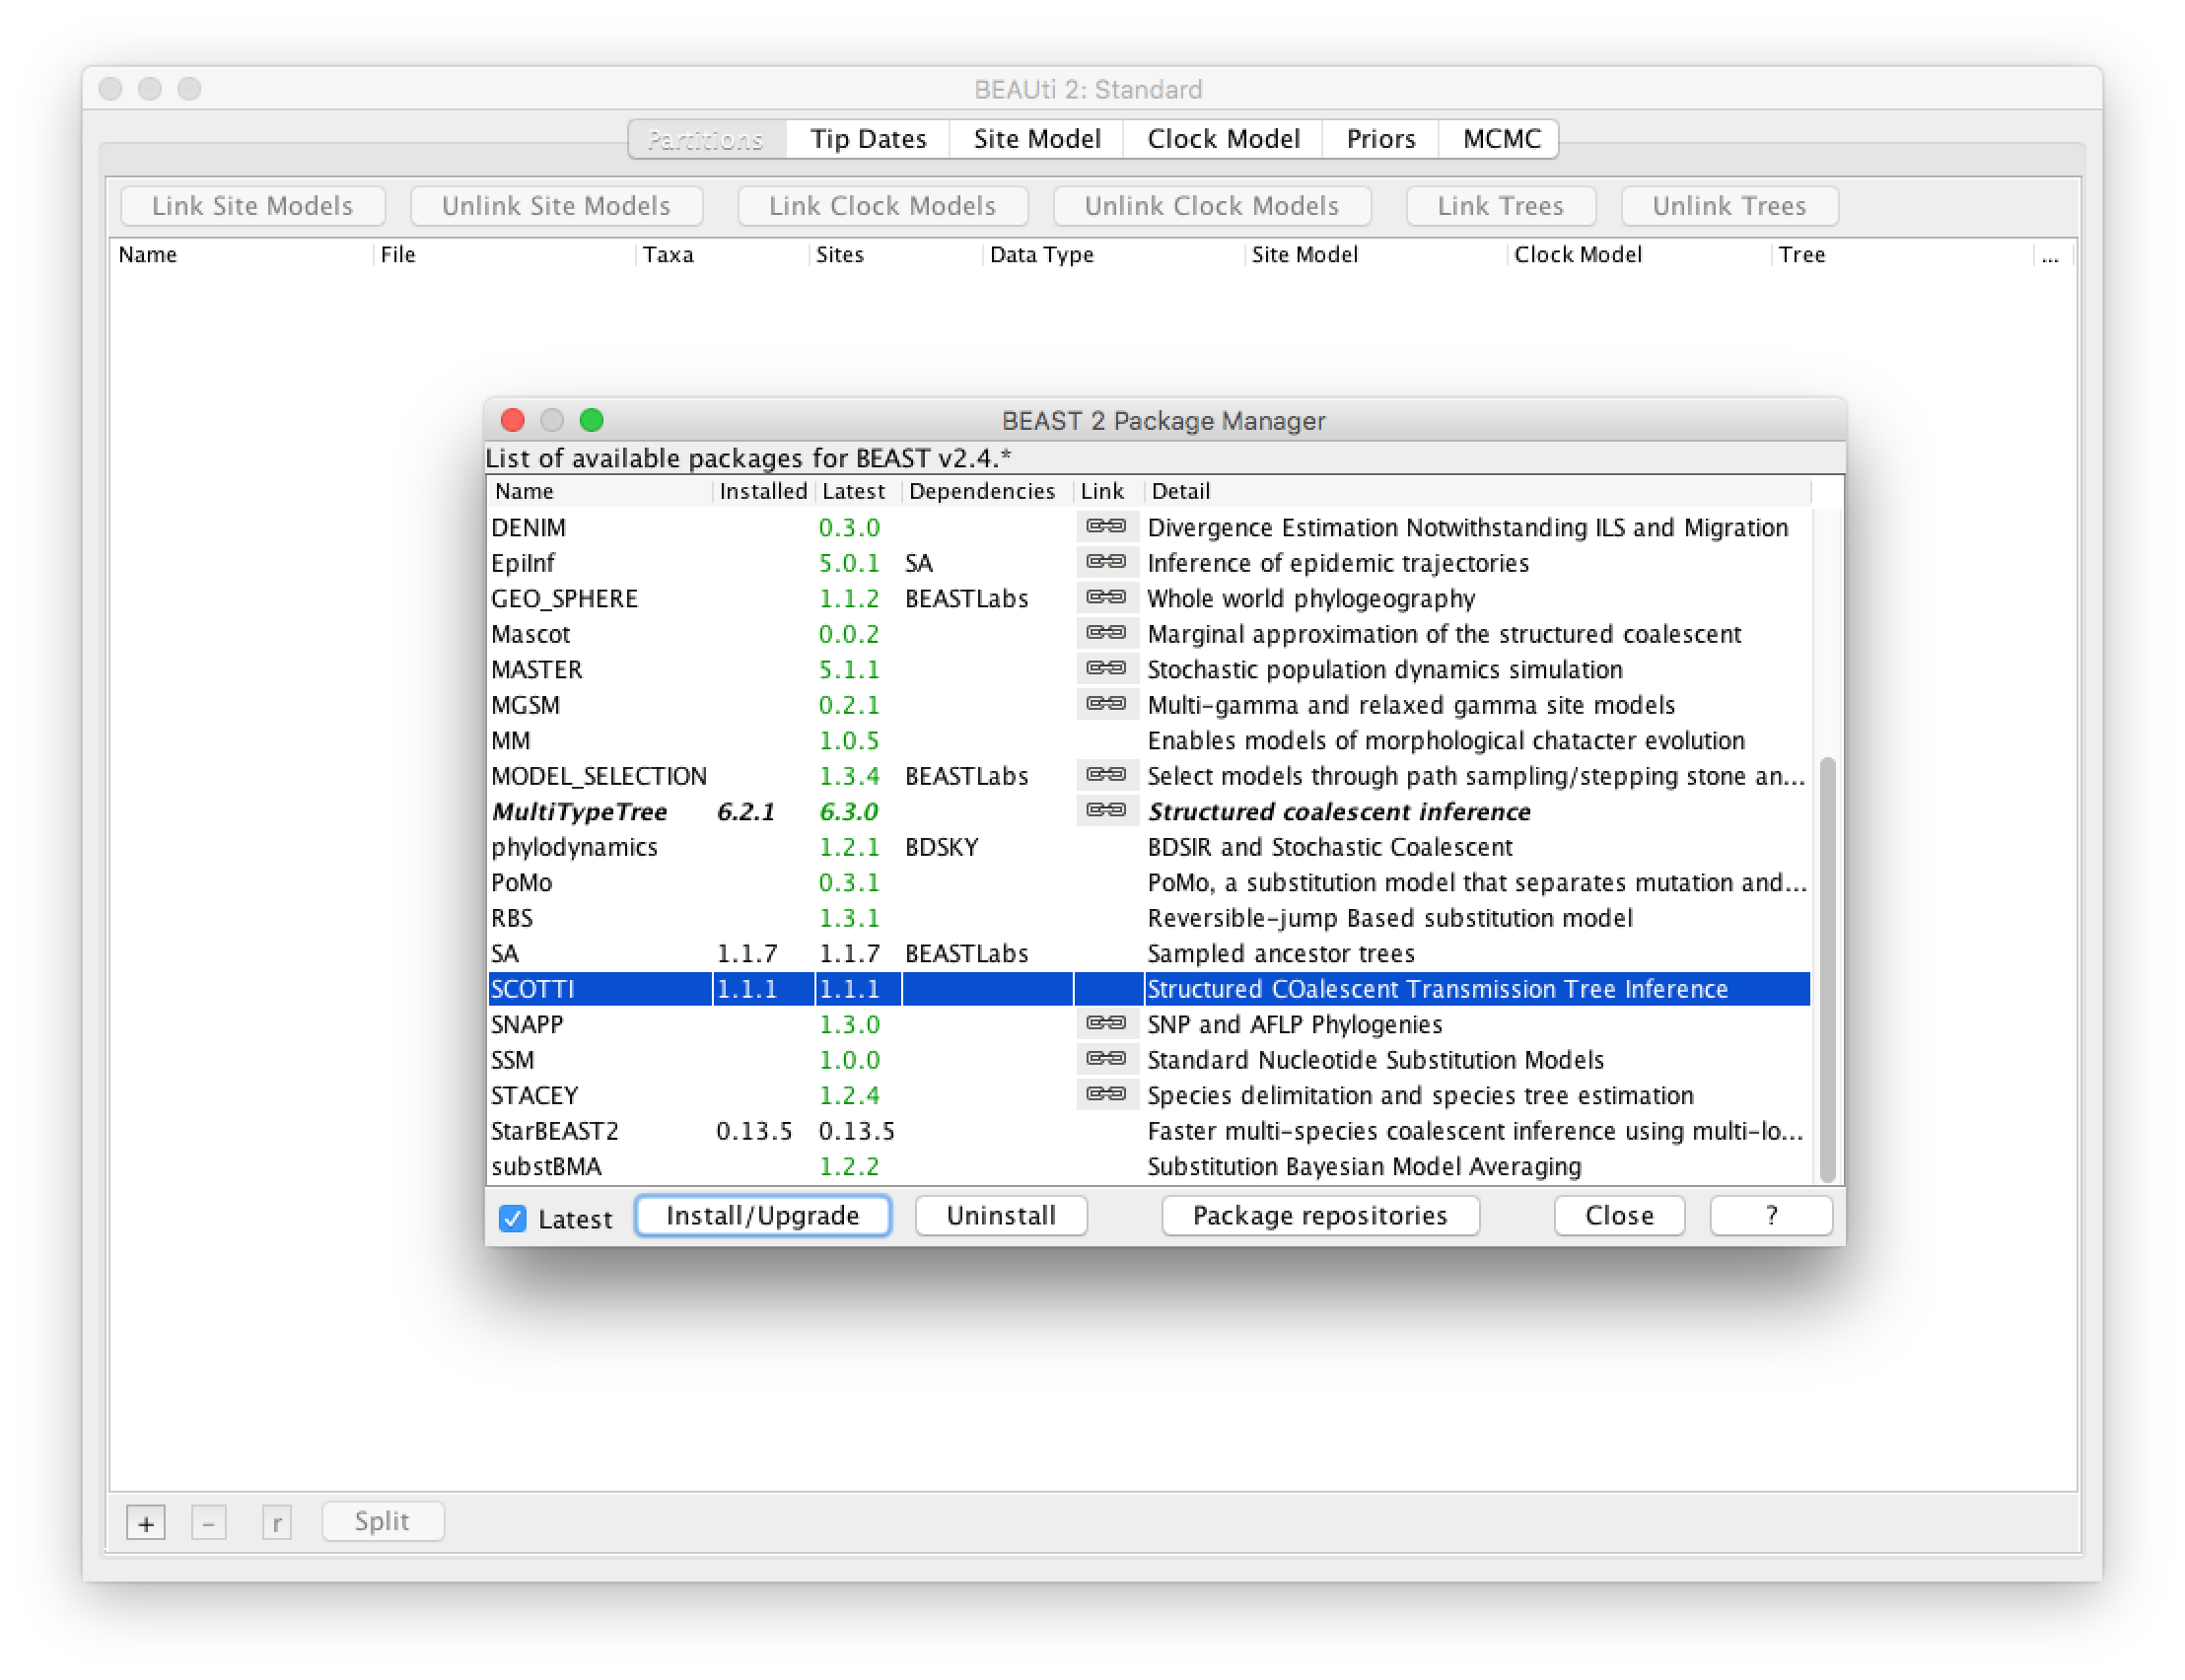
\includegraphics[width=0.800000\textwidth]{figures/PackageManager.png}
    \caption{Installing the SCOTTI package.}
    \label{fig:packagemanager}
\end{figure}

\subsubsection{Running the Python
script}\label{running-the-python-script}

\begin{framed}
Open a terminal if you are using Mac OS X or Linux, or a Command Prompt
if you are using Windows.

Navigate to the directory where the \lstinline!SCOTTI_generate_xml.py!
script is stored.

Type \lstinline!python SCOTTI_generate_xml.py --help!
\end{framed}

This will display help for the different input arguments of the script:

\begin{lstlisting}[language=bash]

usage: SCOTTI_generate_xml.py [-h] [--fasta FASTA] [--output OUTPUT]
                              [--overwrite] [--dates DATES] [--hosts HOSTS]
                              [--hostTimes HOSTTIMES] [--maxHosts MAXHOSTS]
                              [--unlimLife] [--penalizeMigration]
                              [--numIter NUMITER]
                              [--mutationModel MUTATIONMODEL]
                              [--fixedAs FIXEDAS] [--fixedCs FIXEDCS]
                              [--fixedGs FIXEDGS] [--fixedTs FIXEDTS]
                              [--tracelog TRACELOG] [--screenlog SCREENLOG]
                              [--treelog TREELOG]

optional arguments:
  -h, --help            show this help message and exit
  --fasta FASTA, -f FASTA
                        Input fasta alignment. If not specified, looks in th
                        working directory for SCOTTI_aligment.fas
  --output OUTPUT, -o OUTPUT
                        output file that will contain the newly created SCOTTI
                        xml to be run with BEAST2.
  --overwrite, -ov      Overwrite output files.
  --dates DATES, -d DATES
                        Input csv file with sampling dates associated to each
                        sample name (same name as fasta file). If not
                        specified, looks for SCOTTI_dates.csv
  --hosts HOSTS, -ho HOSTS
                        Input csv file with sampling hosts associated to each
                        sample name (same name as fasta file). If not
                        specified, looks for SCOTTI_hosts.csv
  --hostTimes HOSTTIMES, -ht HOSTTIMES
                        Input csv file with the earliest times in which hosts
                        are infectable, and latest time when hosts are
                        infective. Use same host names as those used for the
                        sampling hosts file. If not specified, looks for
                        SCOTTI_hostTimes.csv

  ...
  ...
  ...

  --treelog TREELOG, -tl TREELOG
                        Logging frequency in the tree file.
                        Default=numIter/1000.
\end{lstlisting}

We see that we have to provide the script with four input files:

\begin{itemize}

\item
  A fasta file, containing the genetic sequences.
\item
  A dates file, containing the sampling dates for each sequence.
\item
  A hosts file, containing a mapping from each sequence to the host it
  was sampled from.
\item
  A hostTimes file, containing the earliest and latest dates when hosts
  are infectious. Thus, these dates correspond to the introduction and
  removal of hosts to the outbreak (for instance in a hospital setting
  these dates will correspond to a patient's admission and release
  dates).
\end{itemize}

The dates, hosts and hostTimes files need to be csv-files
(comma-separated values). All dates have to be provided in numbers. All
four input files for the FMDV outbreak are provided in the
\lstinline!data/! directory of this tutorial.

The sequence file:

\begin{lstlisting}

>IP3c-46
-----------------GGTCTCACCCCTAGTAAGCCAACGACAGTCCCTGCGTTGCACTCCACA...
>IP5-51
-----------------GGTCTCACCCCTAGTAAGCCAACGACAGTCCCTGCGTTGCACTCCACA...
>IP8-62
-----------------GGTCTCACCCCTAGTAAGCCAACGACAGTCCCTGCGTTGCACTCCACA...

... 

>IP1b-4
-----------------GGTCTCACCCCTAGTAAGCCAACGACAGTCCCTGCGTTGCACTCCACA...
\end{lstlisting}

The dates file:

\begin{lstlisting}

IP3c-46, 46.0
IP5-51, 51.0
IP8-62, 62.0

...

IP6b-54, 54.0
\end{lstlisting}

The hosts file:

\begin{lstlisting}

IP1b-3, IP1b
IP1b-4, IP1b
IP2b-6, IP2b

...

IP8-62, IP8
\end{lstlisting}

The hostTimes file:

\begin{lstlisting}

IP1b, -26.0, 7.0
IP2b, -16.0, 9.0
IP2c, -9.0, 10.0

...

IP8, 43.0, 63.0
\end{lstlisting}

Note that the script assumes that times are specified forward-in-time,
thus the largest times are the ones closest to the present. In this
analysis we specify time in days from the start of the outbreak (day 0).
Thus, in the hostTimes file, where times are negative, that indicates
that we believe those farms could have been infected weeks before the
outbreak was first detected.

\begin{framed}
Type in:

\lstinline!python SCOTTI_generate_xml.py --fasta ../data/FMDV.fasta  --dates ../data/FMDV_dates.csv --hosts ../data/FMDV_hosts.csv --hostTimes ../data/FMDV_hostTimes.csv --output FMDV --maxHosts 20 --numIter 2000000 --tracelog 2000 --treelog 20000 --screenlog 20000!
\end{framed}

This will create the input XML file for the BEAST2 analysis. You may
have to change the paths to the input files before the command will work
(the \lstinline!--fasta!, \lstinline!--dates!, \lstinline!--hosts! and
\lstinline!--hostTimes! arguments). We also specified the following
additional optional arguments:

\begin{itemize}

\item
  \lstinline!--output!: The name of the output XML file and the
  \lstinline!.log! and \lstinline!.tree! files that will be produced by
  BEAST2.
\item
  \lstinline!--maxHosts!: The maximum number of hosts in the outbreak,
  including observed and unobserved hosts. Since we have data from 10
  farms and no cases were found in any other farms it is unlikely that
  more than 20 farms were infected. We can also make the analysis run
  faster by restricting the maximum number of hosts to a smaller number.
\item
  \lstinline!--numIter!: We restrict the length of the chain to
  2'000'000 states.
\item
  \lstinline!--traceLog!, \lstinline!--treelog!,
  \lstinline!--screenlog!: The frequency at which states are saved in
  the log file and tree files or output to the screen. By default the
  Python script will scale these frequencies to log 10'000 states and
  1'000 trees. Since our chain only includes 2'000'000 states this
  results in states being sampled too frequently which in turn results
  in high auto-correlation between sampled states and low ESS values.
\end{itemize}

\begin{framed}
\textbf{Topic for discussion:} Read the help for the
\lstinline!--unlimLife! and \lstinline!--penalizeMigration! input
arguments to the Python script. Can you figure out what these arguments
do? How do you think setting these arguments to true will affect the
results?
\end{framed}

\subsection{Running the analysis}\label{running-the-analysis}

We should now be ready to run the analysis in BEAST2.

\begin{framed}
Open \textbf{BEAST2} and choose \lstinline!FMDV.xml! as the BEAST XML
file. If BEAGLE is installed check the box to use it. Then click
\textbf{Run} (Figure \ref{fig:beastmcmc}).
\end{framed}

\begin{figure}
    \centering
    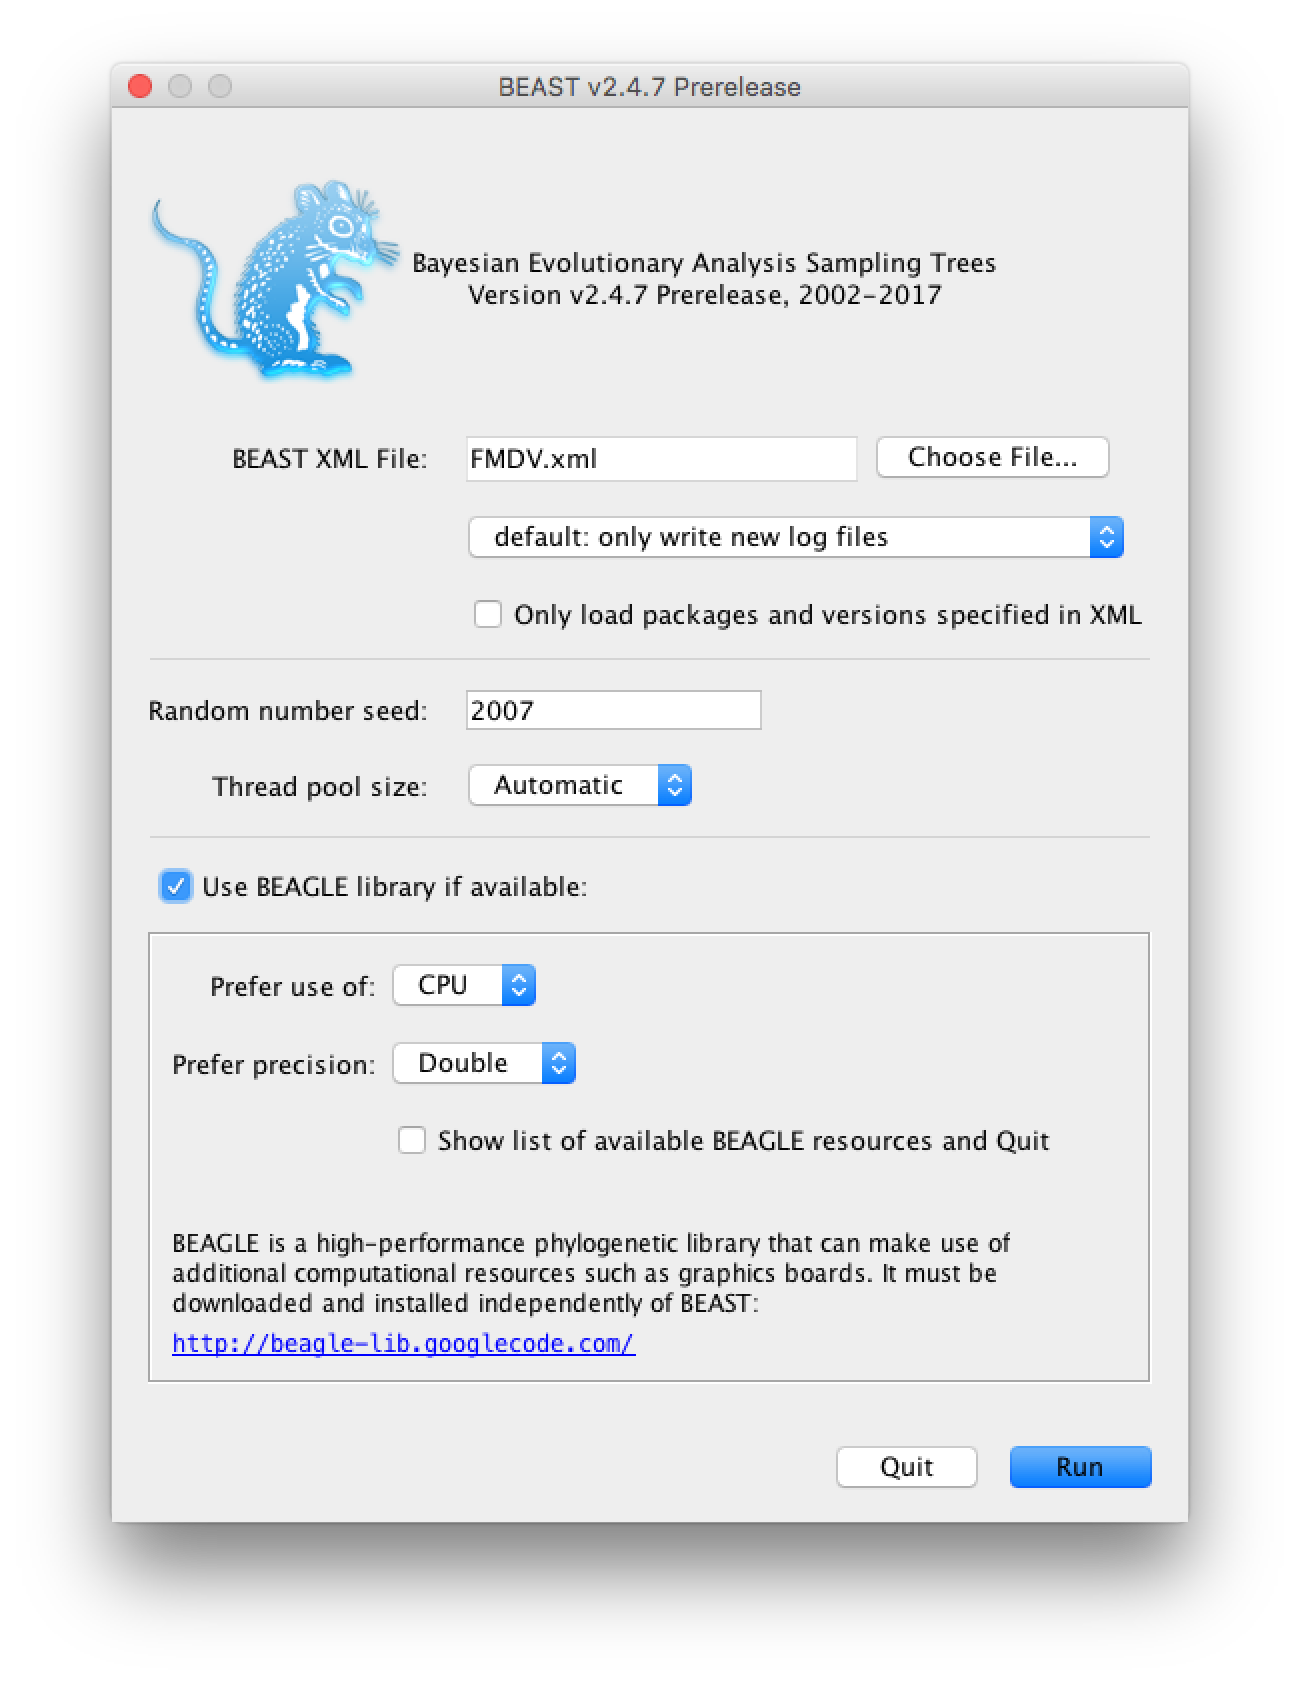
\includegraphics[width=0.500000\textwidth]{figures/BEASTMCMCseed.png}
    \caption{Running the analysis in BEAST2.}
    \label{fig:beastmcmc}
\end{figure}

If you use the seed 2007 you should be able to duplicate the results in
the next section. The analysis should take between 10 and 20 minutes to
run. While the analysis is running open the XML file in a text editor
and see if you can identify the different model components.

\begin{framed}
\textbf{Topic for discussion:} The Python script we used to create the
configuration file only allows us to choose between a Jukes-Cantor or
HKY site model, without any rate heterogeneity or invariant sites. In
addition, it only allows one locus/partition in the alignment and uses a
strict clock. It also doesn't give us any options for setting different
priors or operators.

Do you think there are situations where you would want to use a
different site or clock model? What about the model priors? In
particular, which priors would you want to change?

Suppose you wanted to perform a SCOTTI analysis using a GTR substitution
with a lognormal relaxed clock. How would you go about it?
\end{framed}

\subsection{Analysing the output in Tracer and
FigTree}\label{analysing-the-output-in-tracer-and-figtree}

\begin{framed}
Open \textbf{Tracer} and load the file \lstinline!FMDV.log!. Click on
the \textbf{Trace} tab and examine the parameter traces.
\end{framed}

The Python script only logs a few key parameters (Figure
\ref{fig:tracer}). Note that not all parameters have perfect mixing. For
a real analysis we would run the chain much longer and aim to collect at
least 10'000 samples (this log file contains only 1'000 samples).

\begin{figure}
    \centering
    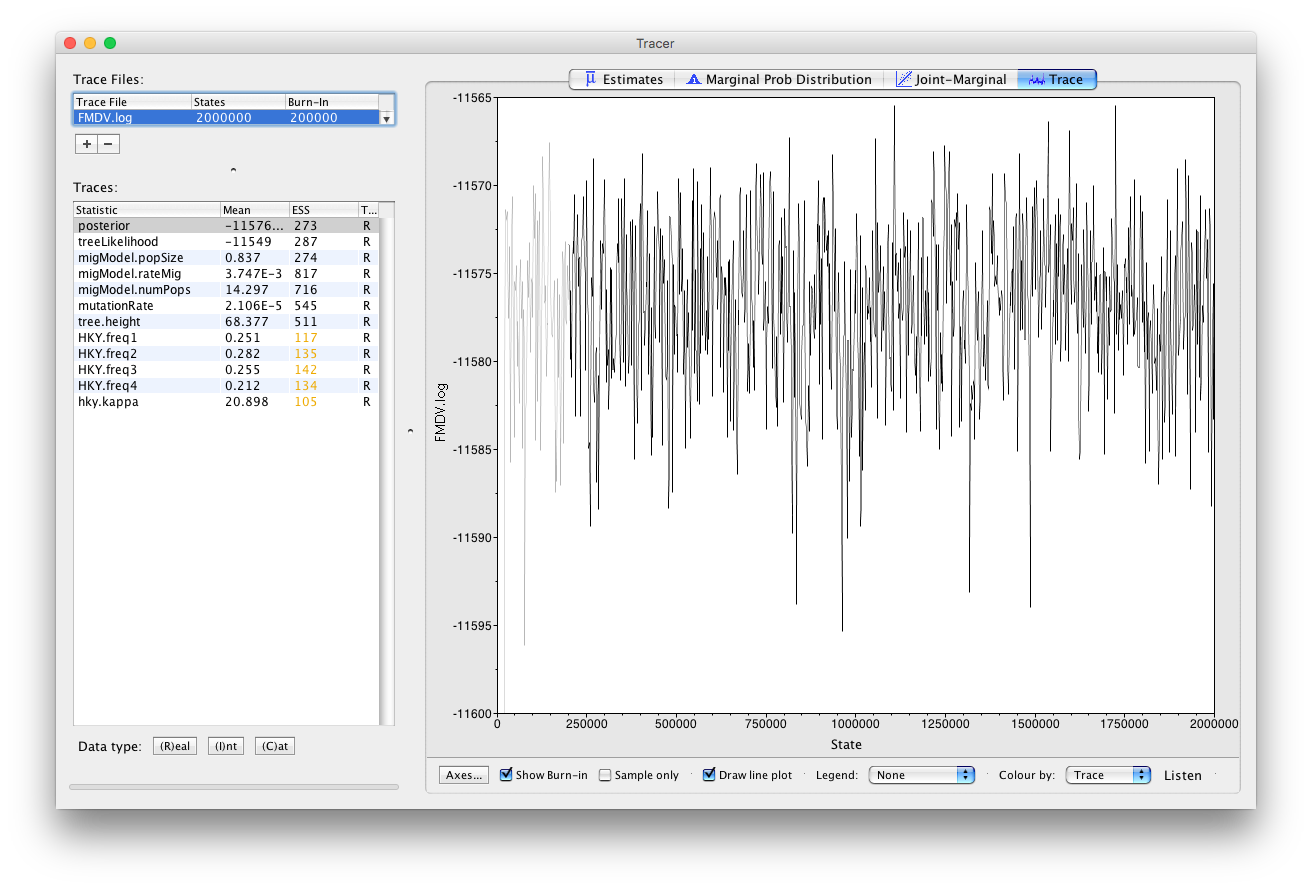
\includegraphics[width=0.800000\textwidth]{figures/Tracer.png}
    \caption{The results of the analysis in Tracer.}
    \label{fig:tracer}
\end{figure}

\begin{framed}
Click on \textbf{Estimates} and select \textbf{migmodel.numPops}.

Since this is an integer parameter click on \textbf{(I)nt} at the bottom
of the panel (Figure \ref{fig:numPops}).
\end{framed}

\begin{figure}
    \centering
    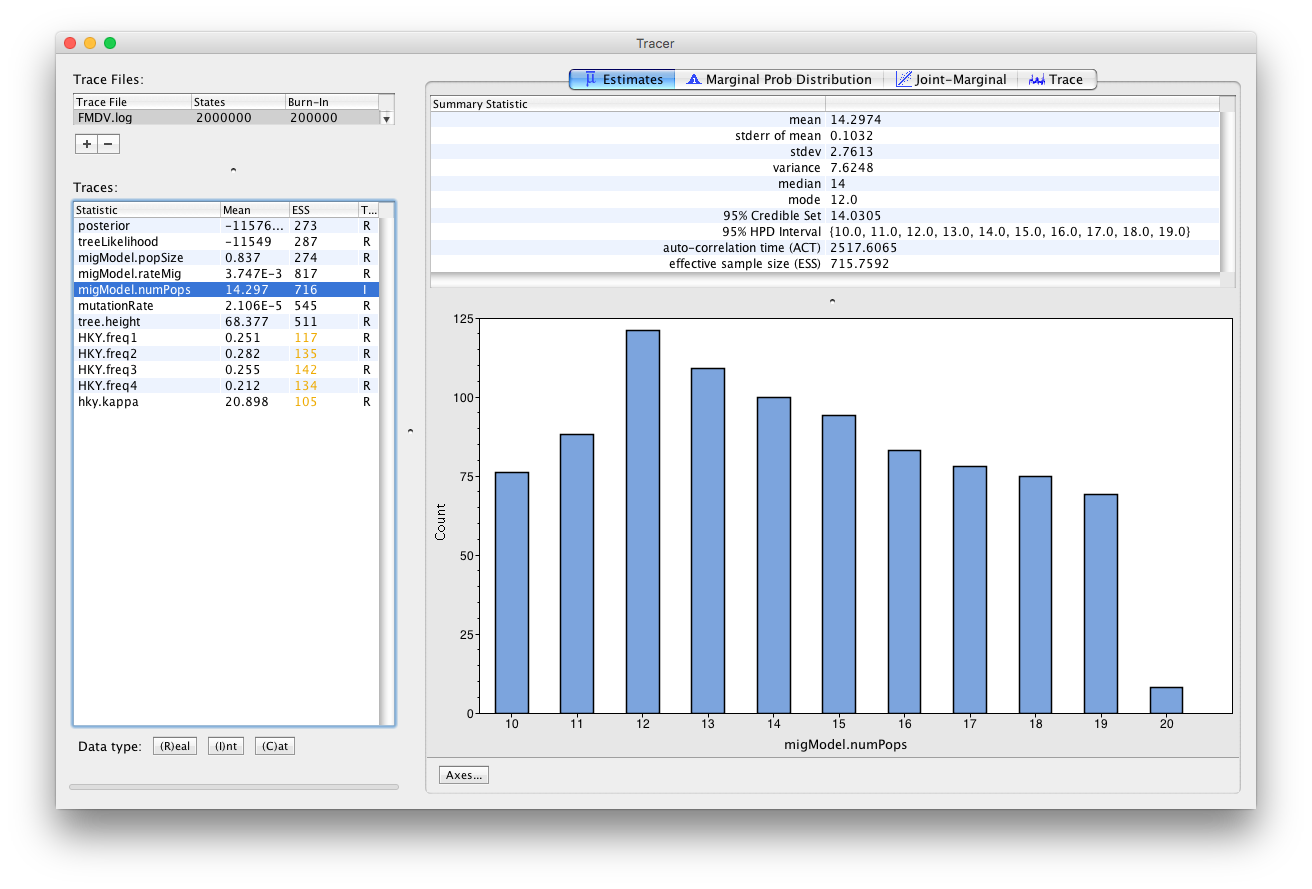
\includegraphics[width=0.800000\textwidth]{figures/Tracer_numPops.png}
    \caption{Estimates for the number of infected farms.}
    \label{fig:numPops}
\end{figure}

This parameter estimates the number of hosts in the outbreak. It is
bounded below by 10 (the number of sampled farms) and above by 20, which
was our input upper bound. However, it is difficult to interpret this
parameter as the number of farms that were infected, because (i) one
non-sampled deme may actually represent a series of hosts with no time
overlap, or a single host with unlimited exposure time (like
environmental contamination); (ii) non-sampled hosts are not necessarily
infected; (iii) many non-sampled hosts might just represent one host
with large population size, like an environmental endemic source.

The parameter \textbf{migModel.popSize} logs the effective population
size of the hosts, which is directly proportional to the genetic
diversity of the virus within each farm. We see that the effective
population size is quite low, which is probably due to the relatively
short period of the outbreak. The equal infection rate between farms is
logged by \textbf{migModel.rateMig} and the clock rate by
\textbf{mutationRate}. If the clock rate seems low for a virus, keep in
mind that we measure time in days. Thus, the units for substitutions are
in substitutions/site/day instead of the usual substitutions/site/year.

\begin{framed}
Select \textbf{tree.height} (Figure \ref{fig:tmrca})
\end{framed}

\begin{figure}
    \centering
    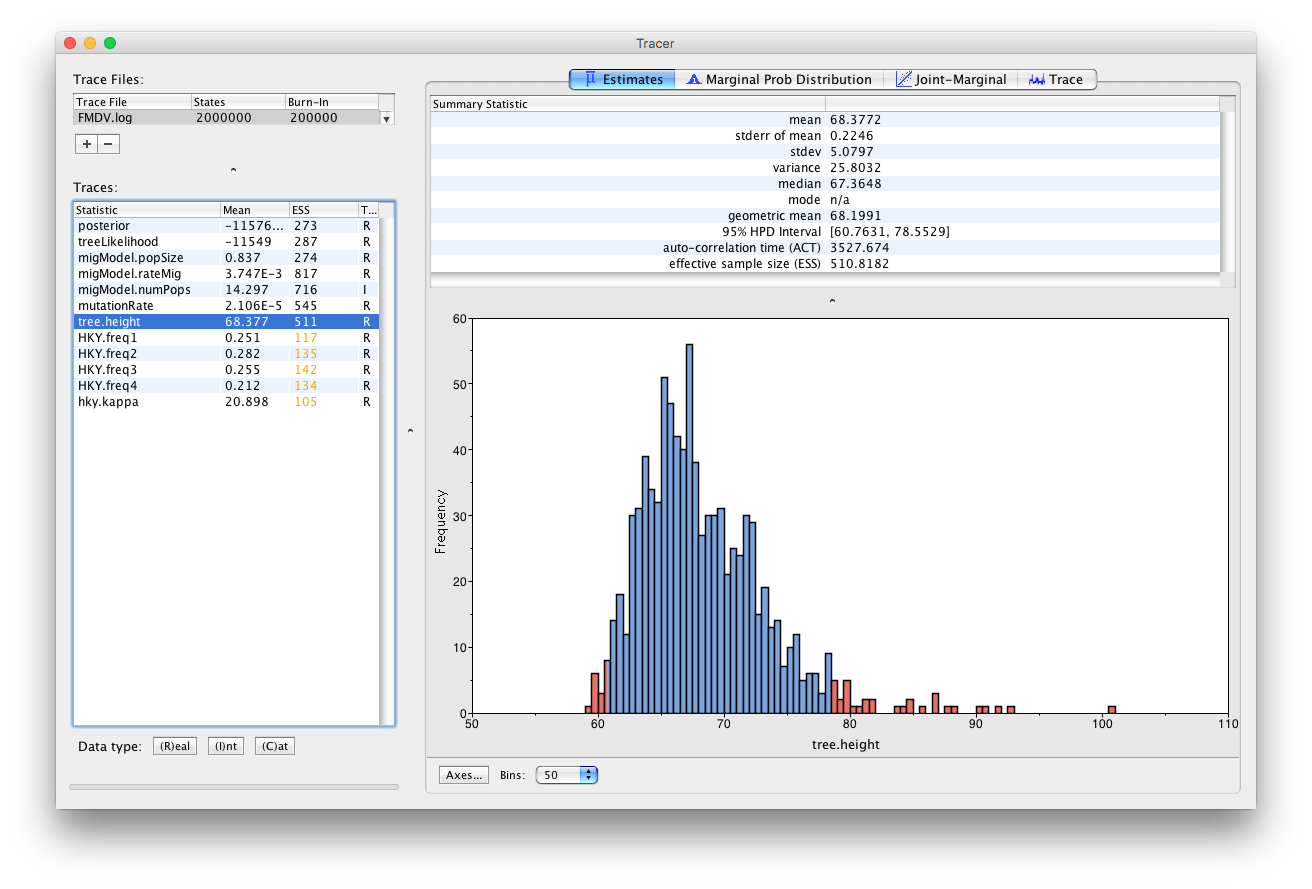
\includegraphics[width=0.800000\textwidth]{figures/Tracer_TMRCA.png}
    \caption{Estimates for the TMRCA.}
    \label{fig:tmrca}
\end{figure}

This parameter is the TMRCA of the sequences included in the
transmission tree. The median estimate is 67.36 days, with a 95\% HPD
between 60.76 and 78.55 days. Since the most recent sample was taken on
day 62 of the outbreak (IP8-62), this indicates that it is unlikely that
the outbreak started more than a week before it was discovered and
confirmed, which is an encouraging sign for the surveillance of foot and
mouth disease in the United Kingdom.

\begin{framed}
Open \textbf{TreeAnnotator} and set the \textbf{Burnin percentage} to
10. Leave the other options unchanged.

Load the file \lstinline!FMDV.trees! and change the \textbf{Output file}
to \lstinline!FMDV.MCC.tree! (Figure \ref{fig:treeannotator}).
\end{framed}

\begin{figure}
    \centering
    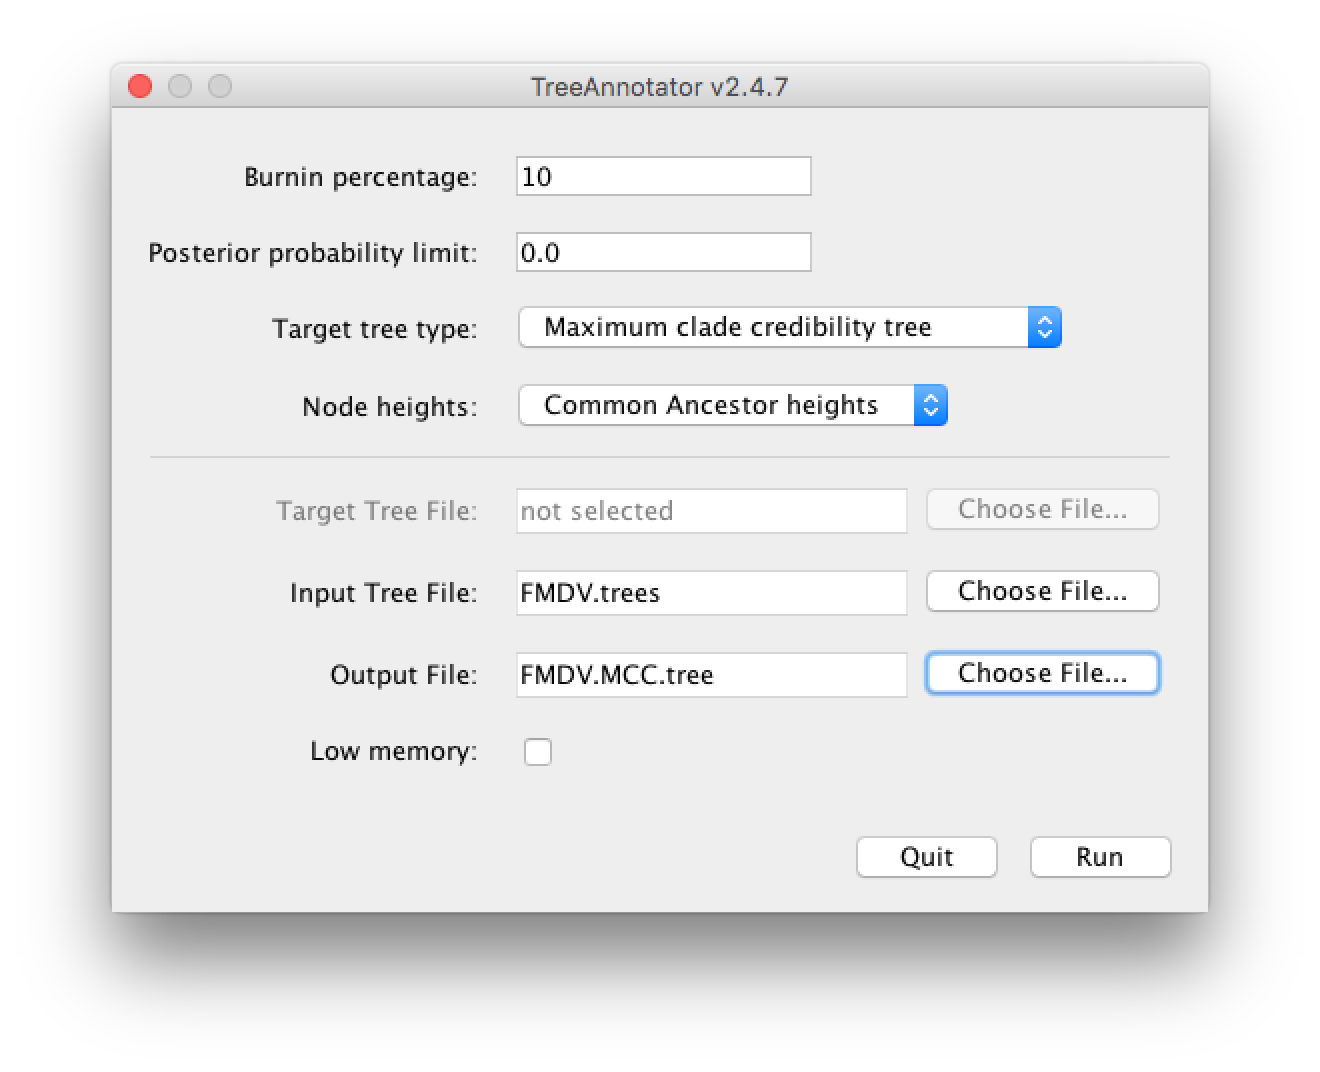
\includegraphics[width=0.500000\textwidth]{figures/TreeAnnotator.png}
    \caption{Creating the MCC tree.}
    \label{fig:treeannotator}
\end{figure}

\begin{framed}
Open \textbf{FigTree} and load \lstinline!FMDV.MCC.tree!.

Click on the arrow to the right \textbf{Appearance} and in the
\textbf{Colour by} dropdown box select \textbf{host}. Check
\textbf{Gradient} and increase the \textbf{Line Weight} to \textbf{5}.

Increase the \textbf{Font Size} under \textbf{Tip Labels} and change
\textbf{Display} to \textbf{host}. Check \textbf{Node Labels} and select
\textbf{host.prob} from the dropdown box and increase the \textbf{Font
size}.

Under \textbf{Node Shape} select \textbf{Circle} and set the size by
\textbf{host.prob} and the colour by \textbf{host}.

Check \textbf{Legend} and select \textbf{host} as \textbf{Attribute}.
\end{framed}

\begin{figure}
    \centering
    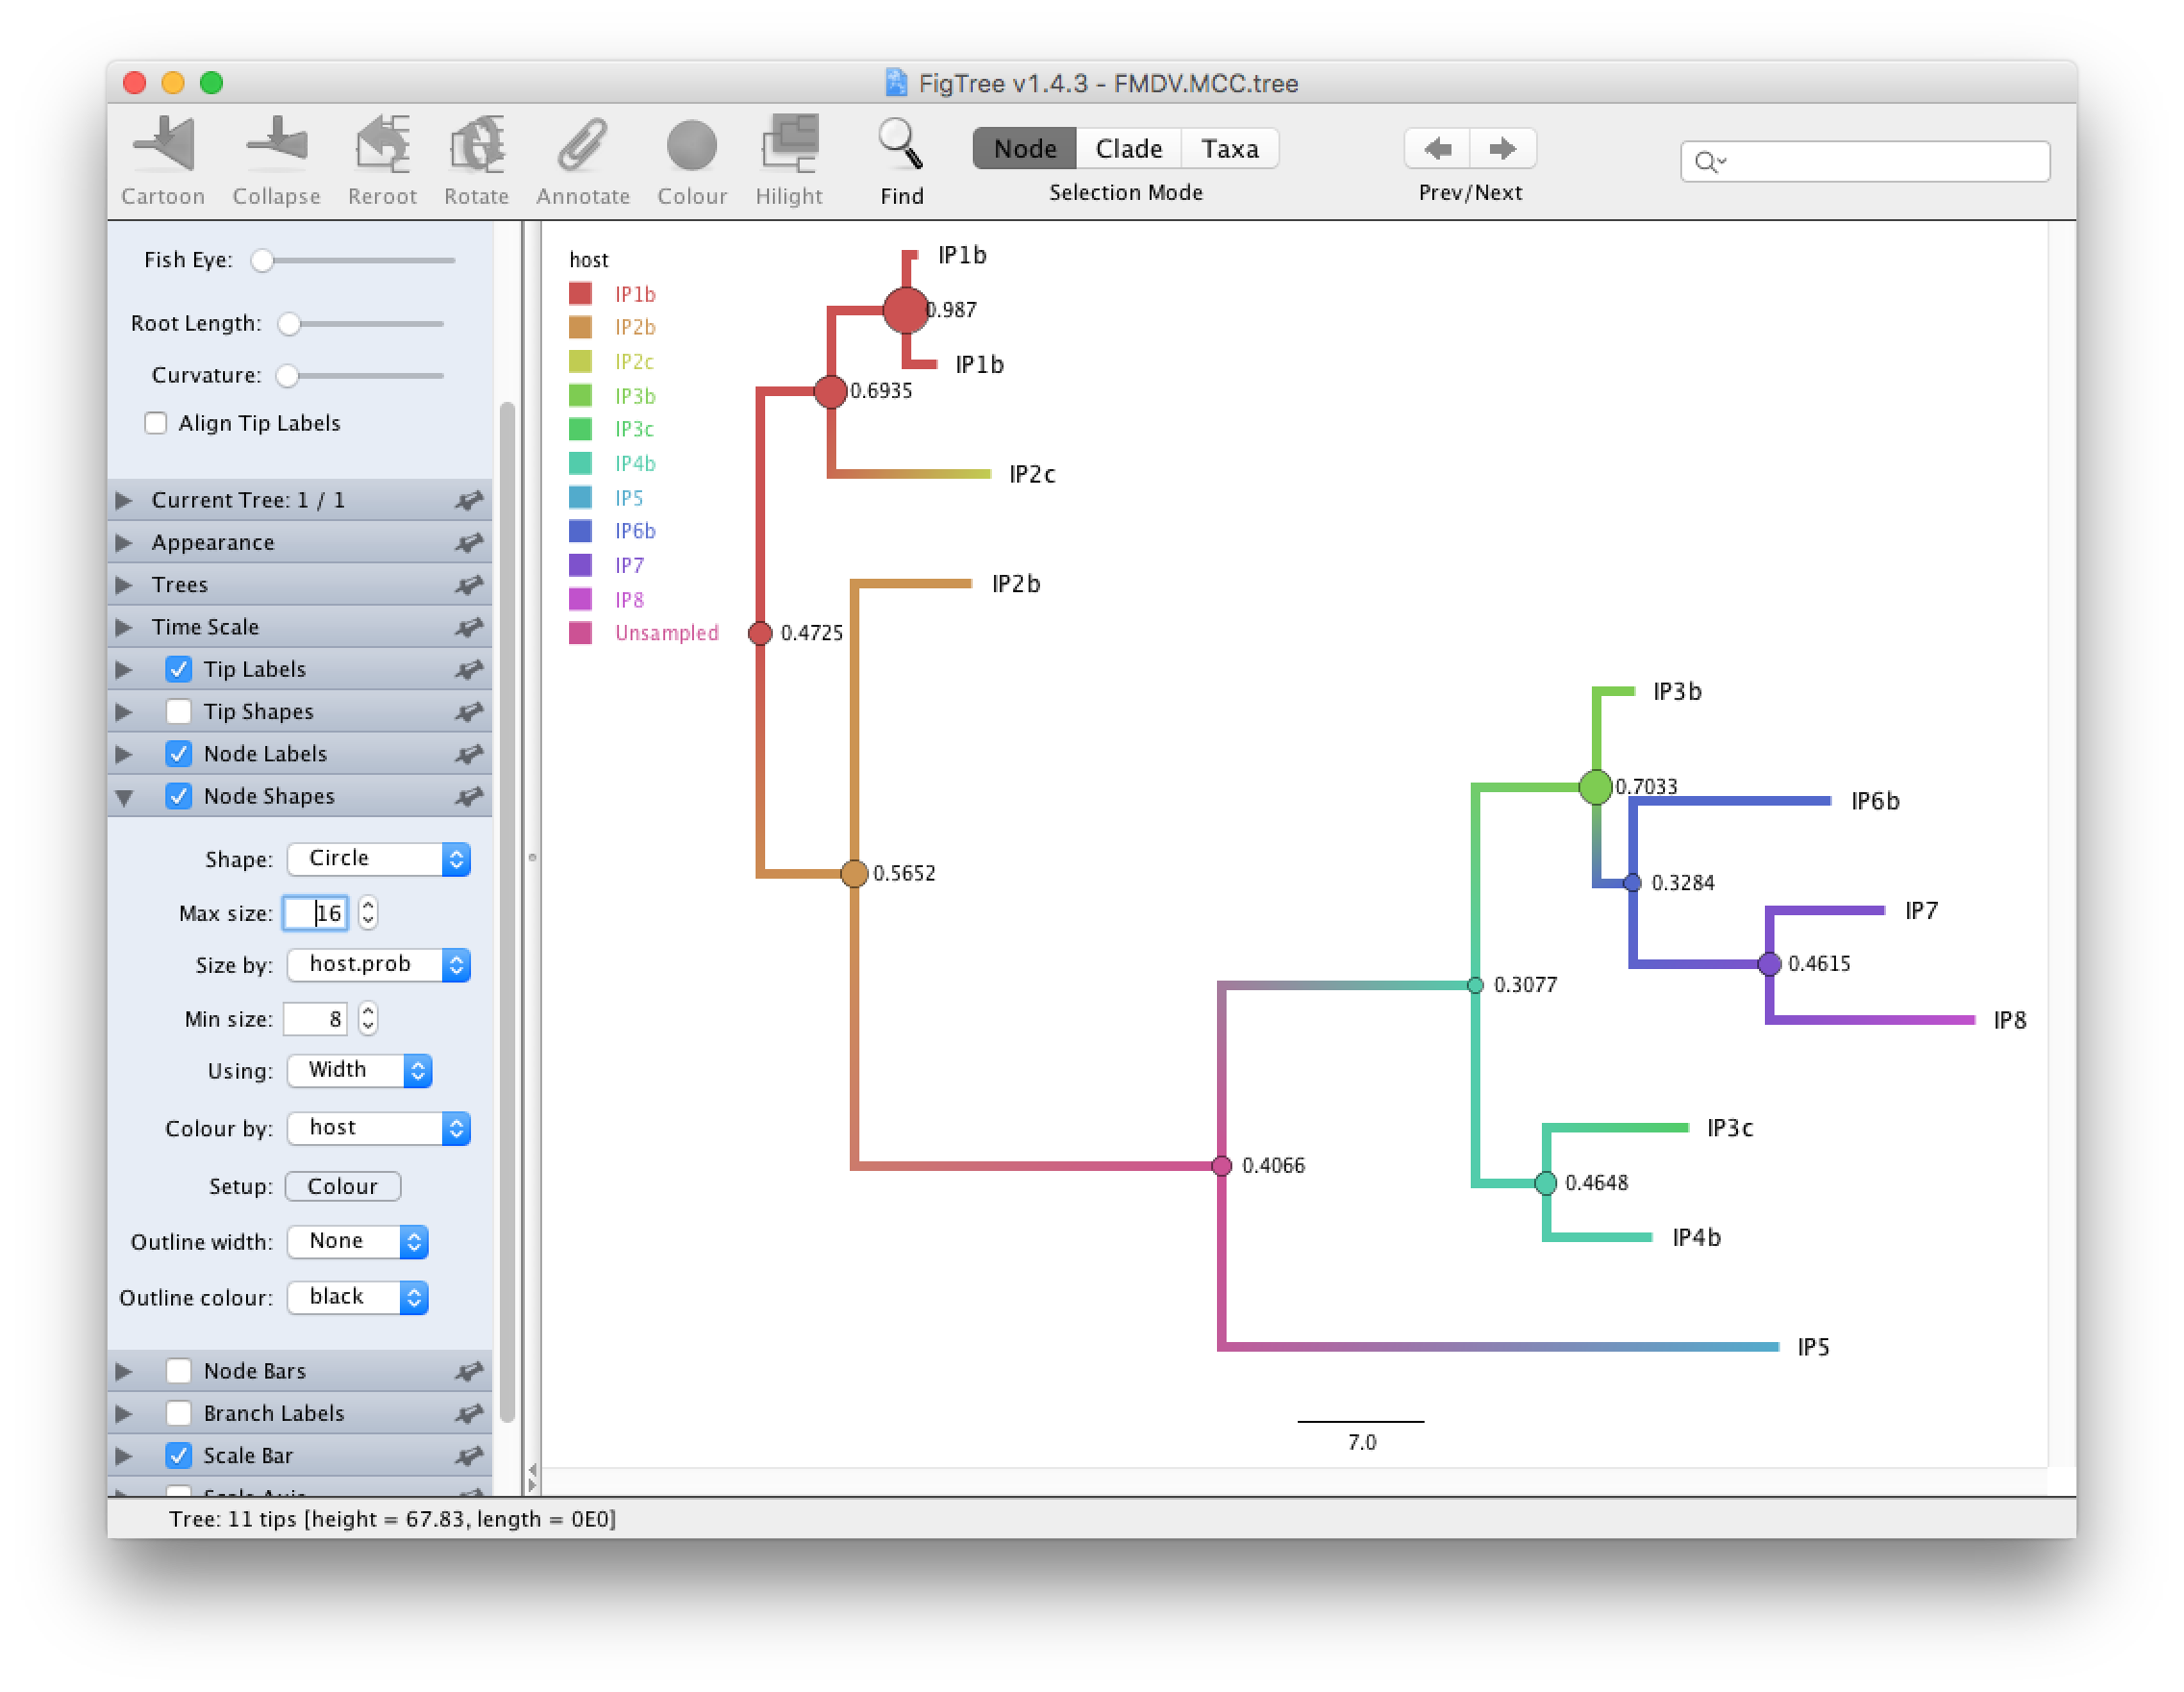
\includegraphics[width=1.000000\textwidth]{figures/FigTree.png}
    \caption{The MCC tree in FigTree.}
    \label{fig:figtree}
\end{figure}

We see that in the MCC tree (Figure \ref{fig:figtree}) one node is an
unsampled node (between the two outbreak clusters). Thus, there is
evidence of a non-sampled farm between IP2b and IP5. We further see that
while the posterior probabilities for some internal nodes are quite
high, it is below 0.5 for several nodes. Note that since SCOTTI does not
model the transmission bottleneck it cannot estimate the time of
infection. Thus, it is better to display the tree with a gradient
between hosts than with a discrete colouring.

\begin{framed}
Under \textbf{Node Labels} change the \textbf{Display} attribute first
to \textbf{host.set} and then to \textbf{host.set.prob} (Figure
\ref{fig:hostsets})
\end{framed}

\begin{figure}
    \centering
    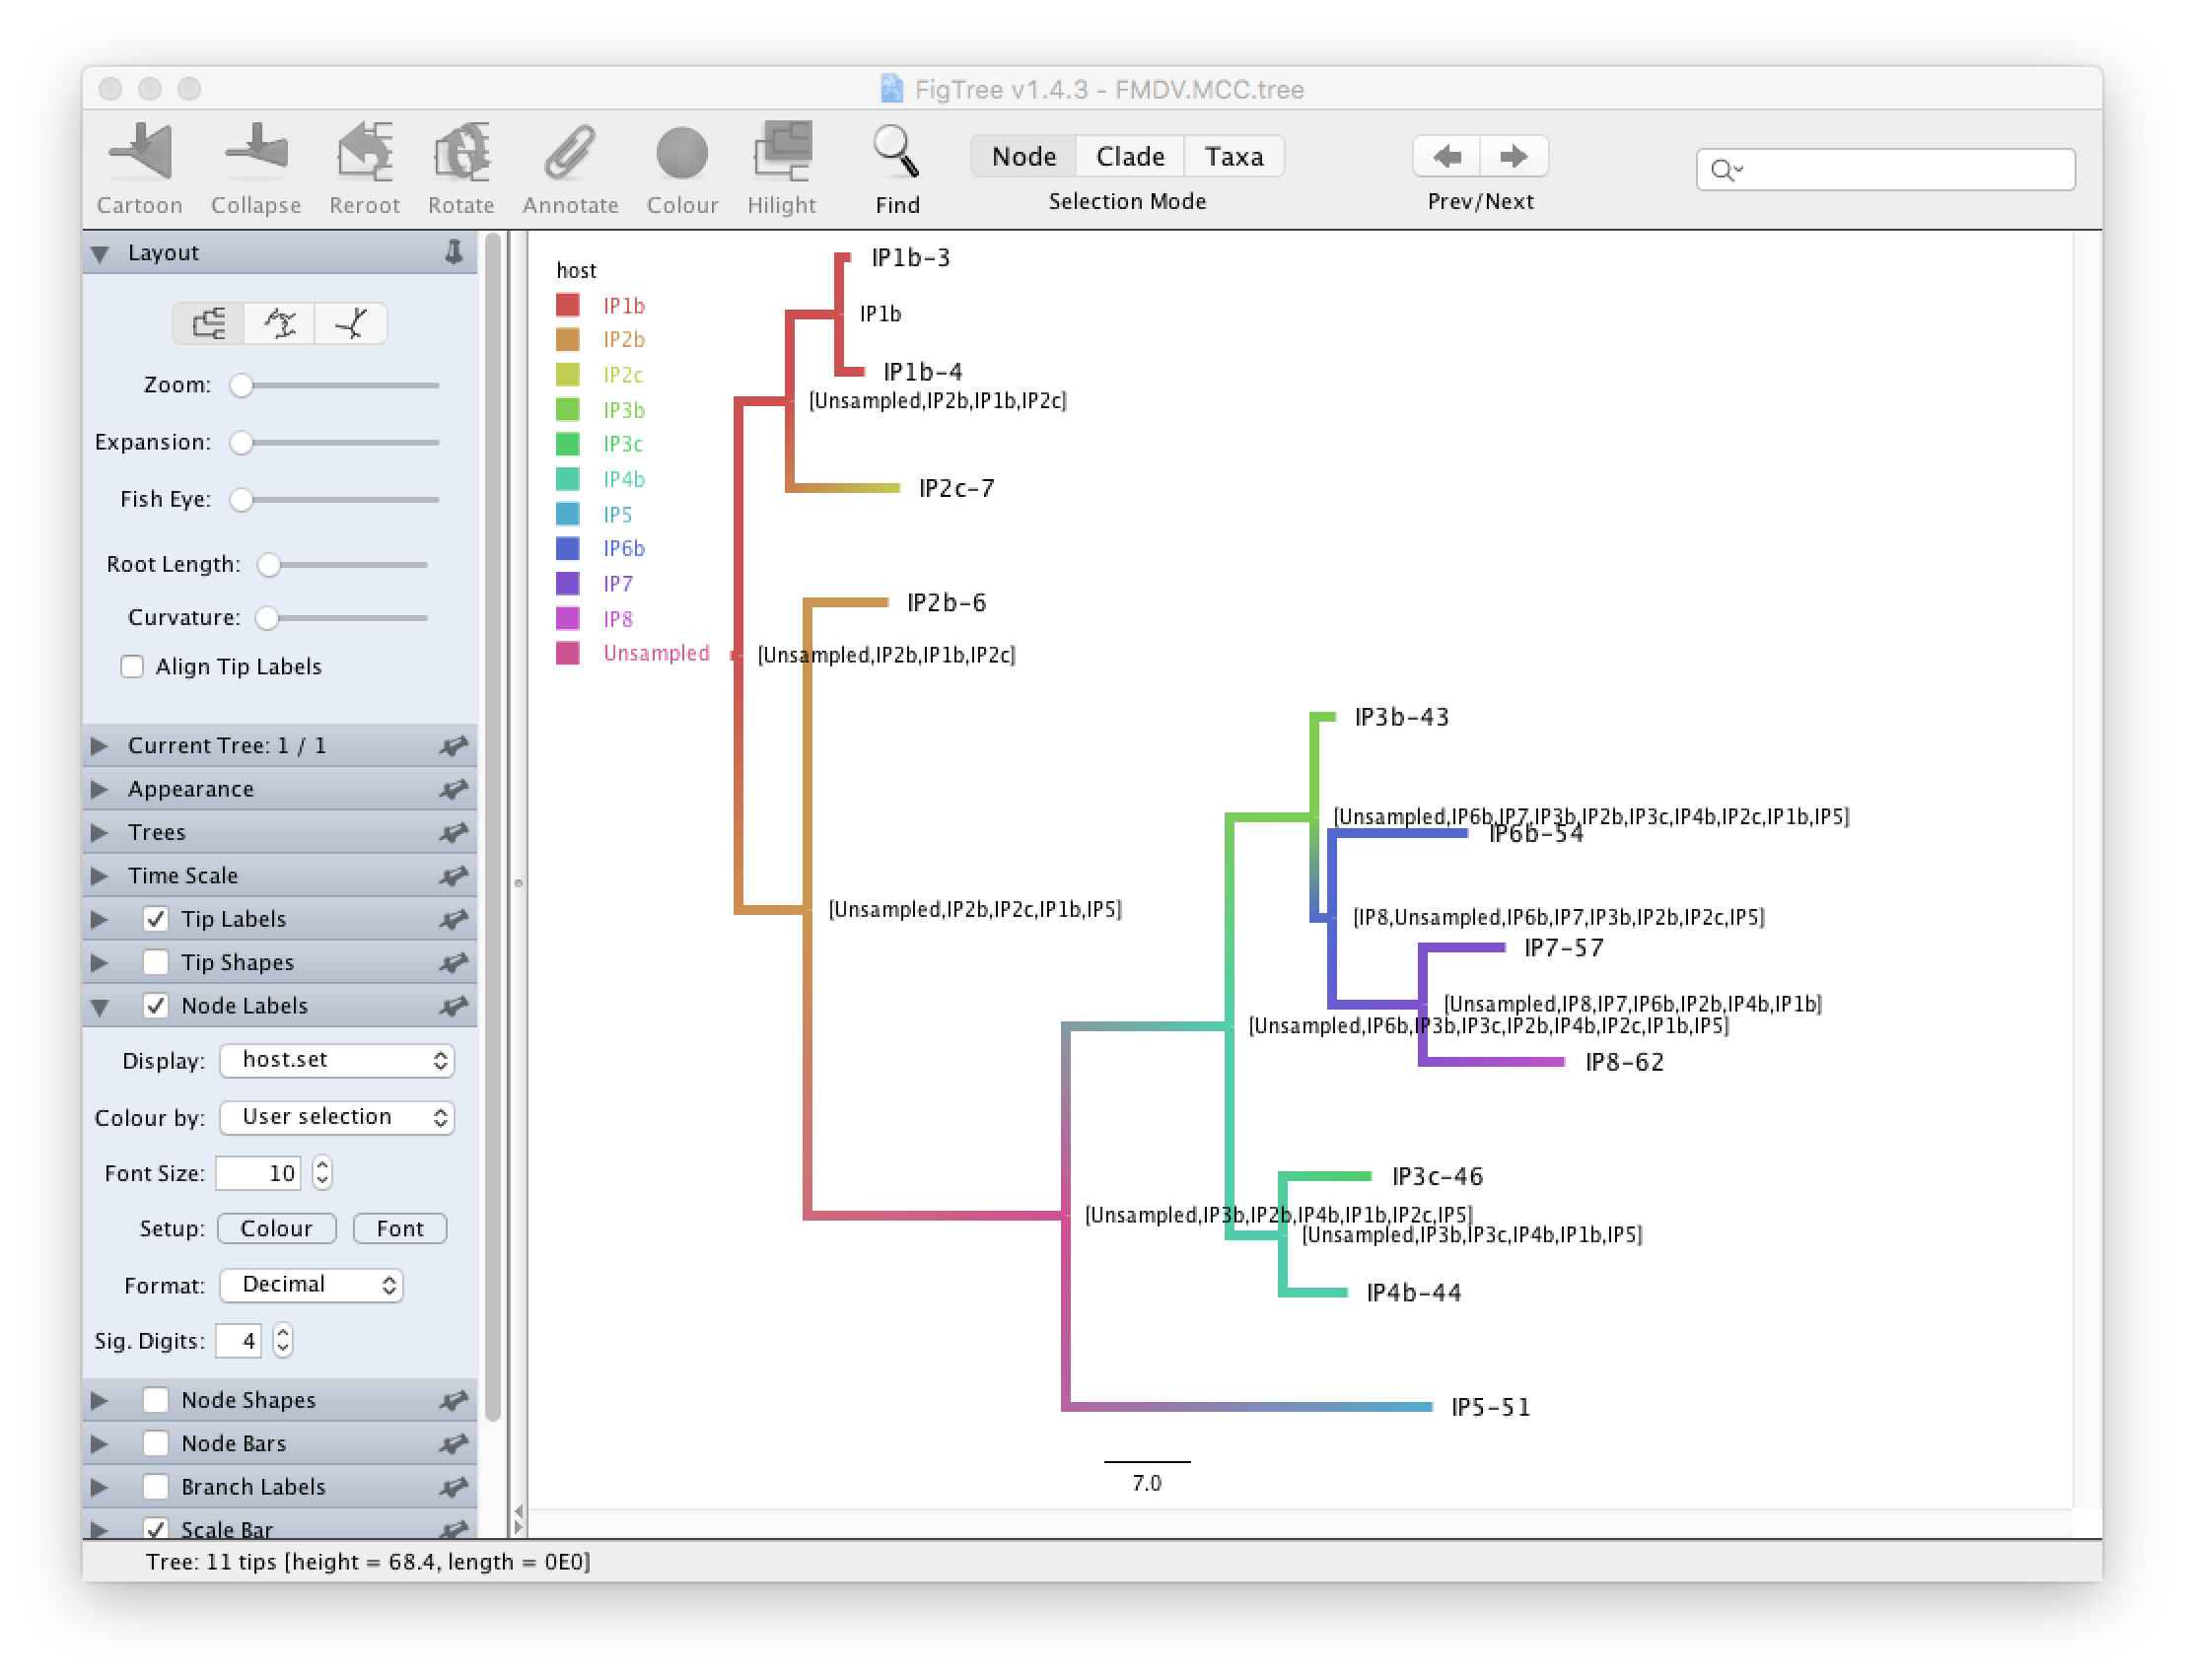
\includegraphics[width=1.000000\textwidth]{figures/FigTreeSet.png}
    \caption{The sets of probable hosts in FigTree.}
    \label{fig:hostsets}
\end{figure}

This displays respectively the set of hosts with a non-zero posterior
probability and the posterior probability for those nodes. We see that
although many internal nodes have a large set of possible hosts, only
two or three hosts have reasonably large posterior probabilities for
each internal node.

\subsection{Constructing the transmission
network}\label{constructing-the-transmission-network}

The MCC tree is a summary of the set of posterior trees. Although it is
useful it is not necessarily the best way to look at the transmission
tree. We will use a Python script to construct a transmission network
that shows the probabilities of transmissions between every pair of
farms. We will use the script
\lstinline!Make_transmission_tree_alternative.py!, which uses the
\lstinline!graphviz! package. If this package is not installed you will
have to install it, either through Homebrew or by installing the
Anaconda Python distribution. Alternatively, if you have previously
installed the \lstinline!graph-tool! package you may use the script
\lstinline!Make_transmission_tree.py!, which will produce better looking
figures.

\begin{framed}
Open a terminal if you are using Mac OS X or Linux, or a Command Prompt
if you are using Windows.

Navigate to the directory where the
\lstinline!Make_transmission_tree_alternative.py! script is stored.

Type in
\lstinline!python Make_transmission_tree_alternative.py --input ../precooked_runs/FMDV.trees --outputF FMDV_transmission --burnin 10!
\end{framed}

This will create 3 files:

\begin{itemize}

\item
  \lstinline!FMDV_transmission_direct_transmissions.jpg!
\item
  \lstinline!FMDV_transmission_indirect_transmissions!
\item
  \lstinline!FMDV_transmission_network.txt!
\end{itemize}

\begin{figure}
    \centering
    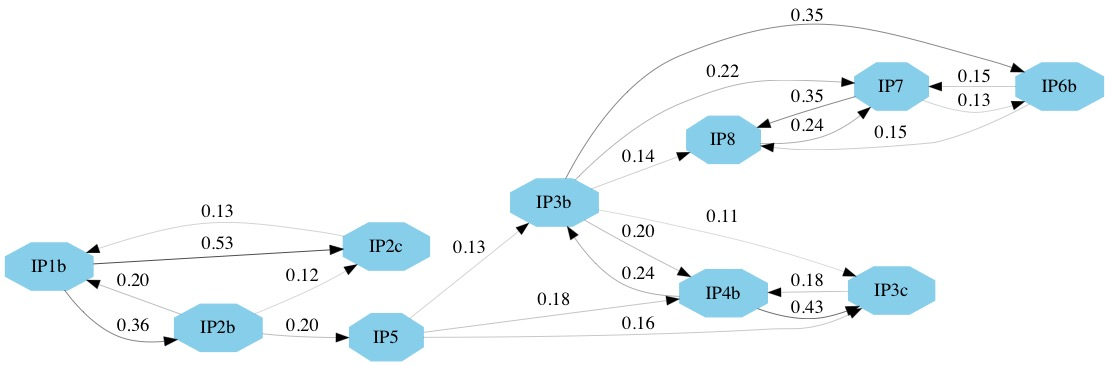
\includegraphics[max width=\textwidth, max height=0.9\textheight]{figures/FMDV_transmission_direct_transmissions.jpg}
    \caption{The direct transmission network using graphviz.}
    \label{fig:hostsets}
\end{figure}

\begin{figure}
    \centering
    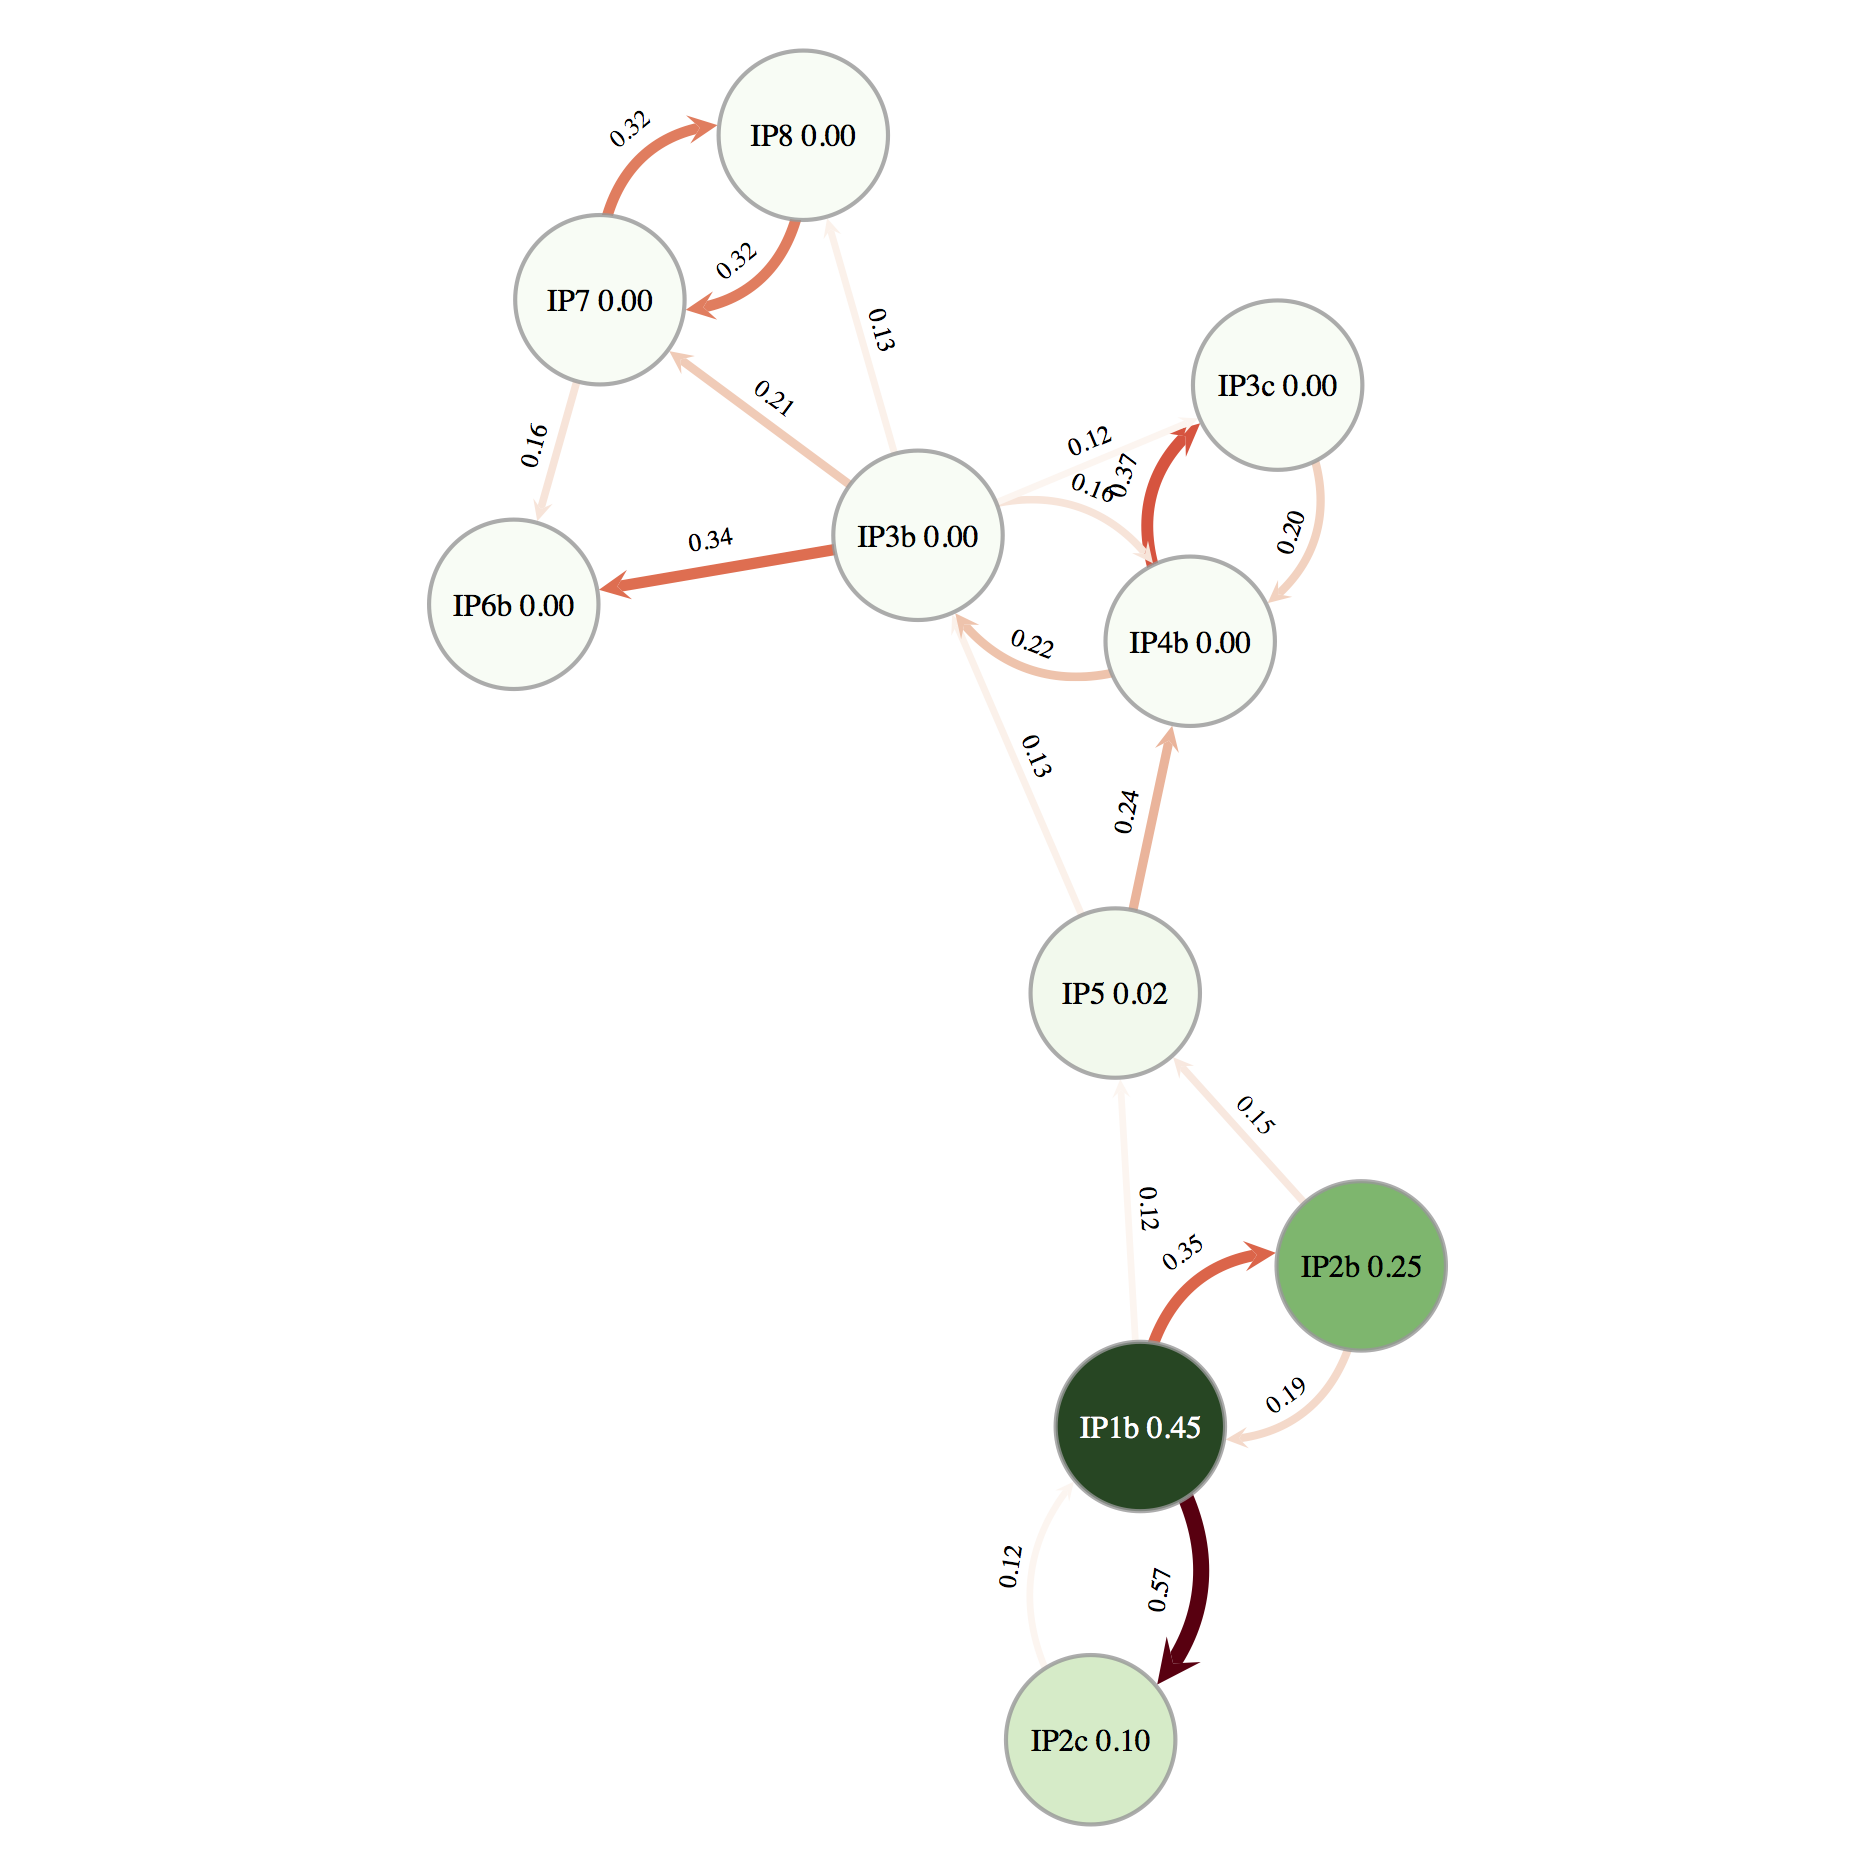
\includegraphics[max width=\textwidth, max height=0.9\textheight]{figures/FMDV3_out_direct_transmissions.png}
    \caption{The direct transmission network using graph-tool.}
    \label{fig:hostsets}
\end{figure}

The network of direct transmissions is shown in
\href{fig:transmissiontree1}{Figure 10}. By default only transmissions
with a probability bigger than 10\% are shown. We can identify a few key
points from the transmission network. First, the chance of a direct
transmission between the first and the second cluster (betwen IP2b and
IP5) is quite low, thus there is a large chance that there are some
non-sampled farms. There also appears to be evidence for non-sampled
farm(s) between IP5 and the other farms in the second cluster. Secondly,
it appears likely that IP3b was responsible either directly or
indirectly, for the infection of IP6b, IP7 and IP8. In several parts of
the network there are a number of possible transmission routes, however
in most cases one route is more likely than others. For example, it is
more likely that IP1b infected IP2c and that IP7 infected IP8 than
vice-versa. It also appears likely that IP1b was the first infected
farm. This information is also summarised in the text file
\lstinline!FMDV_transmission_network.txt!.

Although this information is very useful for informing us about the
transmission dynamics of an outbreak we should be careful not to
over-interpret the results. There is still a lot of uncertainty in the
transmission network, thus a link in the network does not necessarily
indicate a definite transmission pair. Moreover, the presence of
non-sampled hosts make it difficult to unambiguously identify
transmission pairs or superspreaders.

\clearpage

\section{Useful Links}\label{useful-links}

\begin{itemize}

\item
  SCOTTI website with documentation:
  \url{https://bitbucket.org/nicofmay/scotti/}
\item
  \href{http://www.beast2.org/book.html}{Bayesian Evolutionary Analysis
  with BEAST 2} \citep{BEAST2book2014}
\item
  BEAST 2 website and documentation: \url{http://www.beast2.org/}
\item
  Join the BEAST user discussion:
  \url{http://groups.google.com/group/beast-users} 
\end{itemize}



%%%%%%%%%%%%%%%%%%%%%%%
% Tutorial disclaimer %
%%%%%%%%%%%%%%%%%%%%%%%
% Please do not change the license
% Add the author names and relevant links
% Add any other aknowledgments here
\href{http://creativecommons.org/licenses/by/4.0/}{
\includegraphics[scale=0.8]{figures/ccby.pdf}} This tutorial was written by Louis du Plessis and Nicola de Maio for \href{https://taming-the-beast.github.io}{Taming the BEAST} and is licensed under a \href{http://creativecommons.org/licenses/by/4.0/}{Creative Commons Attribution 4.0 International License}. 


%%%%%%%%%%%%%%%%%%%%
% Do NOT edit this %
%%%%%%%%%%%%%%%%%%%%
Version dated: \today




%%%%%%%%%%%%%%%%
%  REFERENCES  %
%%%%%%%%%%%%%%%%

\printbibliography[heading=relevref]


\end{document}